%fig 6.9 p287 missing

\باب{غیر تابع وقت نظریہ اضطراب}\شناخت{باب_غیر_تابع_وقت_نظریہ_اضطراب}

\حصہ{ غیر انحطاطی نظریہ اضطراب}
\جزوحصہ{ عمومی ضابطہ  بندی}
فرض کریں ہم کسی مخفیہ (مثلاً   یک  بعدی لامتناہی چوکور کنویں) کے لئے غیر تابع وقت مساوات شروڈنگر:
\begin{align}\label{مساوات_اضطراب_پہلی}
H^0\psi_n^0=E_n^0\psi_n^0
\end{align}
حل کر کے معیاری عمودی امتیازی تفاعلات \عددی{\psi_n^0} کا مکمل سلسلہ
\begin{align}
\langle \psi_n^0 | \psi_m^0 \rangle = \delta_{nm}
\end{align}
اور ان کی مطابقتی امتیازی اقدار \عددی{E_n^0} حاصل کرتے ہیں۔ اب ہم مخفیہ میں معمولی اضطراب پیدا کرتے ہیں (مثلاً کنویں کی تہہ میں ایک چھوٹا موڑا ڈال کر؛  شکل \حوالہ{شکل_غیر_تابع_اضطراب_چکور_معمولی}) ہم  نئے  امتیازی تفاعلات اور امتیازی اقدار جاننا چاہیں گے
\begin{align}\label{مساوات_اضطراب_بنیادی}
H\psi_n = E_n\psi_n
\end{align}
%
\begin{figure}
\centering
\begin{tikzpicture}
\fill[path fading=west,color=lgray] (-0.25,0) rectangle (0,3.75);
\fill[path fading=east,color=lgray] (5,0) rectangle (5.25,3.75);
\draw[-stealth] (-0.5,0) -- (5.75,0)node[below]{$x$};
\draw[-stealth] (0,-0.25) -- (0,4)node[left]{$V(x)$};
\draw[very thick](0,3.75) -- (0,0) -- (3,0) to [out=30,in=180](3.5,0.5) to [out=0,in=150](4,0) -- (5,0)node[below]{$a$} -- (5,3.75);
\end{tikzpicture}
\caption{لامتناہی چوکور کنویں میں معمولی اضطراب}
\label{شکل_غیر_تابع_اضطراب_چکور_معمولی}
\end{figure}

تاہم ہماری  خوش قسمتی کے علاوہ ایسی   کوئی وجہ   نہیں  پائی  جاتی کہ  ہم اس  پیچیدہ مخفیہ کے لیے مساوات شروڈنگر کو بالکل ٹھیک ٹھیک حل کر  پائیں ۔ \اصطلاح{ نظریہ   اضطراب}،      غیر  مضطرب صورت کے معلوم ٹھیک ٹھیک حلوں کو لے کر،  قدم بقدم چلتے ہوئے مضطرب مسئلے کے  \ترچھا{تخمینی}  حل دیتا ہے۔  ہم نئے  ہیملٹنی کو دو اجزاء کا  مجموعہ:
\begin{align}
H = H^0 + \lambda H'
\end{align}
 لکھ کر آغاز کرتے ہیں ، جہاں \عددی{H'} اضطراب ہے (زیر بالا میں \عددی{0} ہمیشہ  غیر  مضطرب مقدار کو ظاہر کرتا ہے)۔  ہم وقتی طور پر \عددی{\lambda} کو ایک چھوٹا عدد تصور کرتے ہیں؛  بعد میں اس کی قیمت کو بڑھا کر ایک \عددی{(1)} کر دی جائے گی،  اور \عددی{H} اصل ہیملٹنی ہو گی۔ اگلے  قدم میں،   ہم \عددی{\psi_n} اور \عددی{E_n} کو \عددی{\lambda} کی طاقتی تسلسل کے صورت میں لکھتے ہیں ۔
\begin{align}
\psi_n &= \psi_n^0 + \lambda\psi_n^1 + \lambda^2\psi_n^2+\cdots \label{مساوات_اضطراب_سائے_این}\\
E_n &= E_n^0 + \lambda E_n^1 + \lambda^2 E_n^2+\cdots \label{مساوات_اضطراب_ای_این}
\end{align} 
یہاں \عددی{n} ویں امتیازی قدر کی قیمت میں \اصطلاح{اول رتبی تصحیح} کو \عددی{E_n^1} ظاہر کرتا ہے جبکہ \عددی{n} ویں امتیازی تفاعل میں \اصطلاح{اول رتبی تصحیح} کو  \عددی{\psi_n^1} ظاہر کرتا ہے؛ اسی طرح \عددی{E_n^2} اور \عددی{\psi_n^2} دوم رتبی تصحیح ہوں گی ،و غیر ه۔ مساوات \حوالہ{مساوات_اضطراب_سائے_این} اور مساوات \حوالہ{مساوات_اضطراب_ای_این} کو مساوات \حوالہ{مساوات_اضطراب_بنیادی} میں پر کر کے 
\begin{multline*}
(H^0 + \lambda H')[\psi_n^0 + \lambda \psi_n^1 + \lambda^2 \psi_n^2 + \cdots]\\
= (E_n^0 + \lambda E_n^1 + \lambda^2 E_n^2 + \cdots)[\psi_n^0 + \lambda \psi_n^1 + \lambda^2 \psi_n^2 + \cdots]
\end{multline*}
یا ( \عددی{\lambda} کے ایک جیسے طاقتوں کو اکٹھا لکھ کر)  درج ذیل لکھا جا سکتا ہے ۔
\begin{multline*}
H^0 \psi_n^0 + \lambda (H^0 \psi_n^1 + H' \psi_n^0) + \lambda^2 (H^0 \psi_n^2 + H' \psi_n^1) + \cdots \\
= E_n^0 \psi_n^0 + \lambda (E_n^0 \psi_n^1 + E_n^1 \psi_n^0) + \lambda^2 (E_n^0 \psi_n^2 + E_n^1 \psi_n^1 + E_n^2 \psi_n^0) + \cdots
\end{multline*}
 کمتر رتبہ \عددی{(\lambda^0)} کی صورت میں\حاشیہد{ہمیشہ کی طرح، طاقتی تسلسل پھیلاو کی یکتائی  ضمانت دیتی ہے کہ  ایک جیسی طاقت کے عددی سر ایک جتنے  ہوں گے۔} اس سے \عددی{H^0 \psi_n^0 = E_n^0 \psi_n^0} حاصل ہوتا ہے،  جو   نئی مساوات نہیں ہے (مساوات \حوالہ{مساوات_اضطراب_پہلی})۔ رتبہ اول \عددی{(\lambda^1)} تک درج ذیل ہو گا ۔
\begin{align}\label{مساوات_اضطراب_رتبہ_اول}
H^0 \psi_n^1 + H' \psi_n^0 = E_n^0 \psi_n^1 + E_n^1 \psi_n^0
\end{align}
رتبہ دوم \عددی{(\lambda^2)} تک درج ذیل ہو گا 
\begin{align}\label{مساوات_اضطراب_رتبہ_دوم}
H^0 \psi_n^2 + H' \psi_n^1 = E_n^0 \psi_n^2 + E_n^1 \psi_n^1 + E_n^2 \psi_n^0
\end{align}
و غیر ه ۔ (رتبہ  پر نظر رکھنے کی غرض سے ہم نے \عددی{\lambda} استعمال کیا؛ اب اس کی کوئی  ضرورت نہیں  لہٰذا اس کی قیمت ایک، \عددی{1}، کر دیں۔)

\جزوحصہ{اول رتبی نظریہ}
مساوات \حوالہ{مساوات_اضطراب_رتبہ_اول} کا \عددی{\psi_n^0} کے ساتھ اندرونی ضرب لیتے ہیں  (یعنی \عددی{(\psi_n^0)^*} سے ضرب دے کر تکمل لیتے ہیں)۔ 
\begin{align*}
\langle \psi_n^0 | H^0 \psi_n^1 \rangle + \langle \psi_n^0 | H' \psi_n^0 \rangle = E_n^0 \langle \psi_n^0 | \psi_n^0 | \psi_n^1 \rangle + E_n^1 \langle \psi_n^0 | \psi_n^0 \rangle
\end{align*}
تاہم \عددی{H^0} ہرمشی ہے لہٰذا
\begin{align*}
\langle \psi_n^0 | H^0 \psi_n^1 \rangle = \langle H^0 \psi_n^0 | \psi_n^1 \rangle = E_n^0 \langle \psi_n^0 | \psi_n^1 \rangle
\end{align*}
 ہو گا،  جو دائیں ہاتھ کے پہلے  جزو کو حدف کرے گا۔مزید  \عددی{
\langle \psi_n^0 | \psi_n^0 \rangle = 1
} 
کی بنا پر درج ذیل ہو گا ۔\حاشیہد{موجودہ سیاق و سباق میں \عددی{\langle\psi_n^0|H'\psi_n^0\rangle} یا   \عددی{\langle\psi_n^0|H'|\psi_n^0\rangle} (جہاں اضافی انتصابی  لکیر شامل کی گئی ہے)  لکھنے میں کوئی فرق نہیں، چونکہ ہم حال کو تفاعل موج کے لحاظ سے "نام"  دیتے ہیں۔لیکن موخر الذکر علامتی اظہار زیادہ بہتر ہے، چونکہ یہ ہمیں اس روایت سے آزاد کرتا ہے۔}
\begin{align}\label{مساوات_غیر_اضطراب_اہم_ترین}
E_n^1 = \langle \psi_n^0 | H' | \psi_n^0 \rangle
\end{align}
یہ رتبہ اول نظریہ اضطراب کا بنیادی نتیجہ ہے؛  بلکہ عملاً یہ پوری کوانٹائی  میکانیات میں غالباً سب سے اہم مساوات ہے۔ یہ کہتی ہے کے  غیر  مضطرب حال میں اضطراب کی توقعاتی قیمت،  توانائی کی  اول رتبی   تصحیح ہو گی۔ 

\ابتدا{مثال}
لامتناہی چوکور کنویں کے غیر مضطرب تفاعلات موج (مساوات \حوالہ{مساوات_شروڈنگر_میری_سائے})   درج ذیل ہیں  ۔
\begin{align*}
\psi_n^0 (x) = \sqrt{\frac{2}{a}} \sin \big (\frac{n \pi}{a} x\big )
\end{align*}
 فرض کریں ہم کنویں کی "تہہ" (زمین)  کو مستقل مقدار \عددی{V_0} اوپر اٹھاتے ہوئے اس نظام کو مضطرب کرتے ہیں (شکل  \حوالہ{شکل_غیر_تابع_اضطراب_چکور_مستقل_اضطراب})۔   توانائیوں میں رتبہ اول  تصحیح تلاش کریں ۔

\begin{figure}
\centering
\begin{tikzpicture}
\fill[path fading=west,color=lgray] (-0.25,0) rectangle (0,3.75);
\fill[path fading=east,color=lgray] (5,0) node[below,black]{$a$} rectangle (5.25,3.75);
\draw[-stealth] (-0.5,0) -- (5.75,0)node[below]{$x$};
\draw[-stealth] (0,-0.25) -- (0,4)node[left]{$V(x)$};
\draw[very thick](0,3.75) -- (0,0.5)node[left]{$V_0$} -- (5,0.5) -- (5,3.75);
\end{tikzpicture}
\caption{پورے کنویں میں مستقل اضطراب}
\label{شکل_غیر_تابع_اضطراب_چکور_مستقل_اضطراب}
\end{figure}

حل: یہاں \عددی{H' = V_0}   ہو گا لہٰذا   \عددی{n} ویں حال کی توانائی میں رتبہ اول تصحیح درج ذیل ہو گی۔
\begin{align*}
E_n^1 = \langle \psi_n^0 | V_0 | \psi_n^0 \rangle = V_0 \langle \psi_n^0 | \psi_n^0 \rangle = V_0
\end{align*}
یوں  تصحیح  شدہ توانائیوں کی سطحیں  \عددی{
E_n \cong  E_n^0 + V_0
} ہوں گی؛ جی ہاں،  تمام  \عددی{V_0} مقدار  اوپر  اٹھتی ہیں۔ یہاں حیرانگی کی بات صرف  یہ ہے کہ رتبہ اول نظریہ بالکل ٹھیک جواب دیتا ہے۔ یوں ظاہر ہے کہ مستقل اضطراب کی صورت میں تمام بلند رتبی تصحیح صفر ہوں گی۔ \حاشیہد{یہاں  کوئی ی چیز لامتناہی چوکور کنویں کی خصوصیات پر منحصر نہیں ہے،  لہٰذا یہی کچھ کسی بھی مخفیہ کے لیے مستقل اضطراب کی صورت میں درست ہو گا۔} اس کے برعکس کنویں کی نصف چوڑائی تک اضطراب کی وسعت کی صورت  (شکل \حوالہ{شکل_غیر_تابع_اضطراب_نصف_چکور_مستقل_اضطراب})  میں درج ذیل   ہو گا۔
\begin{align*}
E_n^1 = \frac{2V_0}{a} \int_0^{a/2} \sin^2 \big(\frac{n \pi}{a} x\big ) \dif  x= \frac{V_0}{2}
\end{align*}
%
\begin{figure}
\centering
\begin{tikzpicture}
\fill[path fading=west,color=lgray] (-0.25,0) rectangle (0,3.75);
\fill[path fading=east,color=lgray] (5,0) rectangle (5.25,3.75);
\draw[-stealth] (-0.5,0) -- (5.75,0)node[below]{$x$};
\draw[-stealth] (0,-0.25) -- (0,4)node[left]{$V(x)$};
\draw[very thick](0,3.75) -- (0,0.5)node[left]{$V_0$} -- (2.5,0.5) -- (2.5,0)node[below]{$\tfrac{a}{2}$} -- (5,0)node[below,black]{$a$} -- (5,3.75);
\end{tikzpicture}
\caption{نصف  کنویں میں مستقل اضطراب}
\label{شکل_غیر_تابع_اضطراب_نصف_چکور_مستقل_اضطراب}
\end{figure}


اب توانائی کی ہر سطح  \عددی{
\frac{V_0}{2}
}
اوپر  اٹھتی ہے۔ یہ غالباً بالکل ٹھیک نتیجہ نہیں،  تاہم  اول رتبی تخمین کے نقطہ نظر سے معقول جواب ہے۔
\انتہا{مثال}

 مساوات  \حوالہ{مساوات_غیر_اضطراب_اہم_ترین}  ہمیں توانائی کی اول رتبی  تصحیح دیتی ہے؛  تفاعل موج کے لئے اول رتبی تصحیح حاصل کرنے کی غرض سے ہم مساوات  \حوالہ{مساوات_اضطراب_رتبہ_اول}  کو درج ذیل روپ میں لکھتے ہے ۔
\begin{align}\label{مساوات_غیر_اضطراب_تصحیح_اول_توانائی}
(H^0 - E_n^0) \psi_n^1 = - (H' - E_n^1) \psi_n^0
\end{align}

چونکہ اس کا دایاں ہاتھ ایک معلوم تفاعل ہے،  لہٰذا یہ \عددی{\psi_n^1} کی  غیر  متجانس  تفرقی مساوات ہے۔  اب غیر مضطرب تفاعلات موج ایک مکمل سلسلہ دیتے ہیں،   لہٰذا   (کسی بھی تفاعل کی طرح)  \عددی{\psi_n^1} کو ان کا خطی جوڑ:
\begin{align}\label{مساوات_غیر_اضطراب_تصحیح_اول_تفاعل}
\psi_n^1 = \sum_{m \ne n} c_m^{(n)} \psi_m^0
\end{align}
 لکھا جا سکتا ہے ۔ اگر \عددی{\psi_n^1} مساوات \حوالہ{مساوات_غیر_اضطراب_تصحیح_اول_توانائی} کو مطمئن کرتے  ہوں تب کسی بھی مستقل \عددی{\alpha} کے لیے \عددی{(\psi_n^1 + \alpha \psi_n^0)} بھی اس مساوات کو مطمئن کریں  گے،   لہٰذا  ہم جزو \عددی{\psi_n^0} کو منفی کر سکتے ہیں؛ ایسا ہی کرتے ہوئے مساوات  \حوالہ{مساوات_غیر_اضطراب_تصحیح_اول_تفاعل}  کے مجموعہ میں \عددی{m = n} شامل نہیں کیا گیا۔ عددی سر \عددی{c_m^{(n)}} تعین کر کے ہم مسئلہ حل کر سکتے ہیں۔
 
  ہم مساوات  \حوالہ{مساوات_غیر_اضطراب_تصحیح_اول_توانائی}  میں مساوات  \حوالہ{مساوات_غیر_اضطراب_تصحیح_اول_تفاعل}  پر کرتے ہوئے، اور  یہ جانتے ہوئے کہ غیر مضطرب مساوات  شروڈنگر   (مساوات \حوالہ{مساوات_اضطراب_پہلی})  کو \عددی{\psi_m^0} مطمئن کرتے ہیں درج ذیل حاصل کرتے ہیں ۔
\begin{align*}
\sum_{m \ne n} {(E_m^0 - E_n^0) c_m^{(n)} \psi_m^0} = - {(H' - E_n^1) \psi_n^0}
\end{align*}
اس کا \عددی{\psi_l^0} کے ساتھ اندرونی ضرب لیتے ہیں ۔
\begin{align*}
\sum_{m \ne n} (E_m^0 - E_n^0) c_m^{(n)} \langle \psi_l^0 | \psi_m^0 \rangle = - \langle \psi_l^0 | H' | \psi_n^0 \rangle + E_n^1 \langle \psi_l^0 | \psi_n^0 \rangle 
\end{align*}
اگر \عددی{l = n} ہو تب بایاں ہاتھ صفر ہو گا اور ہمیں دوبارہ مساوات  \حوالہ{مساوات_غیر_اضطراب_اہم_ترین}  ملتی ہے؛  اگر \عددی{l \ne n} ہو تو 
\begin{align*}
(E_l^0 - E_n^0) c_l^{(n)} = - \langle \psi_l^0 | H' | \psi_n^0 \rangle
\end{align*}
یا 
\begin{align}\label{مساوات_غیر_اضطراب_عددی_سر_ایم}
c_m^{(n)} = \frac{\langle \psi_m^0 | H' | \psi_n^0 \rangle}{E_n^0 - E_m^0}
\end{align}
ہو گا،  لہٰذا ا درج ذیل حاصل ہو گا ۔
\begin{align}\label{مساوات_غیر_اضطراب_تفاعل_این}
\psi_n^1 = \sum_{m \ne n} \frac{\langle \psi_m^0 | H' | \psi_n^0 \rangle}{(E_n^0 - E_m^0)} \psi_m^0
\end{align}
جب تک غیر مضطرب توانائی طیف غیر انحطاطی ہو،   نسب نما  کوئی  مسئلہ کھڑا نہیں کرتا   (چونکہ کسی بھی عددی سر کے لئے  \عددی{m = n} نہیں ہو گا)۔  ہاں  اگر  دو غیر مضطرب حالات کی توانائیاں ایک  جتنی ہوں   ( مساوات  \حوالہ{مساوات_غیر_اضطراب_عددی_سر_ایم}  کے  نسب نما میں صفر پایا جائے گا)  تب نسب نما  ہمیں مصیبت میں ڈالتا ہے؛  ایسی صورت میں \اصطلاح{ انحطاطی نظریہ اضطراب}\فرہنگ{نظریہ اضطراب!انحطاطی}\حاشیہب{degenerate perturbation theory}\فرہنگ{perturbation theory!degenerate} کی ضرورت پیش آئے گی، جس پر حصہ \حوالہ{حصہ_غیر_اضطراب_انحطاطی_نظریہ_اضطراب} میں غور کیا جائے گا۔ 

%KKK 16 jan 2022 edited till here
 یوں اول رتبی  نظریہ اضطراب مکمل ہوتا ہے توانائی کی اول رتبی تصحیح \عددی{E_n^1} مساوات  \حوالہ{مساوات_غیر_اضطراب_اہم_ترین}  دیتی ہے جبکہ تفاعل موج کی اول رتبی  تصحیح \عددی{\psi_n^1} مساوات \حوالہ{مساوات_غیر_اضطراب_تفاعل_این} دیتی ہے میں آپ کو یہاں یہ ضرور بتانا چاہوں گا کہ اگرچہ نظریہ اضطراب عموماً  توانائیوں کی بہت درست قیمتیں دیتا ہے یعنی \عددی{E_n^0 + E_n^1} اصل قیمت \عددی{E_n} کے بہت قریب ہے اس سے حاصل تفاعلات موج عموماً   افسوس  کن  ہوتے ہیں  

\ابتدا{سوال} 
فرض کرے ہم لامتناہی چوکور کنویں کے وسط میں \عددی{\delta} تفاعلی موڑا ڈالتے ہیں 
\begin{align*}
H' = \alpha \delta (x - \frac{a}{2})
\end{align*}
جہاں \عددی{\alpha} ایک مستقل ہے 
\begin{enumerate}[a.]
\item
 اجازتی توانائیوں کی اول رتبی تصحیح تلاش کریں بتائیں کہ جفت \عددی{n} کی صورت میں توانائیاں مضطرب کیوں نہیں ہونگی   
\item
 زمینی حال کی  تصحیح \عددی{\psi_1^1} کی مساوات مساوات 6.13 کو پھیلا کر  ابتدائی تین غیر صفر اجزاء تلاش کریں  
 \end{enumerate}
\انتہا{سوال} 

\ابتدا{سوال}
ہارمونی مرتعش \عددی{[V(x) = \tfrac{1}{2} kx^2]} 
کی اجازتی توانائیاں درج ذیل ہیں 
\begin{align*}
E_n &= \big(n + \frac{1}{2}\big) \hslash \omega  && (n = 0, 1, 2, \cdots )
\end{align*}
جہاں \عددی{
\omega = \sqrt{k/m}
} کلاسیکی تعدد ہے اب فرض کرے مقیاس لچک میں معمولی تبدیلی رونما ہوتی ہے \عددی{k \to (1 + \epsilon ) k}
\begin{enumerate}[a.]
\item
(الف) نئی  توانائیوں کی بالکل ٹھیک ٹھیک قیمتیں  حاصل  کرے (جو یہاں ایک آسان کام ہے)۔ اپنے  کلیہ کو دوم رتبہ تک \عددی{\epsilon} کی طاقتیں تسلسل میں پھیلائیں 
\item
 اب مساوات 6.9 استعمال کرتے ہوئے توانائی میں اول رتبی اضطراب کا حساب لگائیں یہاں \عددی{H'} کیا  ہو گا اپنے نتیجے کا جزو(الف) کے ساتھ موازنہ کرے اشارہ: نئے تکمل کی قیمت کے حصول کی نہ ضرورت اور نہ اجازت ہے 
 \end{enumerate}
\انتہا{سوال} 
\ابتدا{سوال}
ایک لامتناہی چوکور کنویں مساوات 2.19 میں دو یکساں بوسن رکھے جاتے ہیں یہ مخفیہ 
\begin{align*}
V(x_1, x_2) = -aV_0\delta (x_1 - x_2)
\end{align*}
 جہاں \عددی{V_0} ایک مستقل ہے جس کا بعد توانائی ہے  اور \عددی{a} کنویں کی چوڑائی ہے کے ذریعے ایک دوسرے پر بہت معمولی اثر انداز ہوتے ہیں 
\begin{enumerate}[a.]
\item
 پہلی قدم میں ذرات کے باہمی   اثر  کو نظر انداز کرتے ہوئے زمینی حال اور پہلے ہیجان حال کے تفاعلات موج اور مطابقتی توانائیاں تلاش کریں 
\item
 اول رتبی نظریہ اضطراب استعمال کرتے ہوئے زمینی حال اور پہلے    ہیجان  حال کے توانائیوں پر ذرات کے باہمی  اثر کا تخمین اول رتبی نظریہ اضطراب سے دریافت کریں 
 \end{enumerate}
\انتہا{سوال} 

%====================
\جزوحصہ{دوم رتبی توانائیاں}\شناخت{حصہ_غیر_اضطراب_دوم_رتبی_توانائیاں}

یہاں بھی اسی طرح بڑھتے ہوئے ہم \عددی{\psi_n^0} اور دو رتبی مساوات مساوات 6.8 کا اندرونی ضرب لیتے ہیں 
\begin{align*}
\langle \psi_n^0 | H^0 \psi_n^2 \rangle + \langle \psi_n^0 | H' \psi_n^1 \rangle = E_n^0 \langle \psi_n^0 | \psi_n^2 \rangle + E_n^1 \langle \psi_n^0 | \psi_n^1 \rangle + E_n^2 \langle \psi_n^0 | \psi_n^0 \rangle
\end{align*}
یہاں بھی ہم \عددی{H^0} کی ہرمشی پن کو بروئے کار لاتے ہیں 
\begin{align*}
\langle \psi_n^0 | H^0 \psi_n^2 \rangle = \langle H^0 \psi_n^0 | \psi_n^2 \rangle = E_n^0 \langle \psi_n^0 | \psi_n^2 \rangle
\end{align*}
 لہٰذا  بائیں ہاتھ کا پہلا جزو دائیں ہاتھ کے پہلے جزو کے ساتھ کٹ جائے گا   ساتھ   ہی \عددی{
\langle \psi_n^0 | \psi_n^0 \rangle = 1
} ہو گا   لہٰذا  ہمارے پاس \عددی{E_n^2} کا درج ذیل  کلیہ رہ جاتا ہے 
\begin{align}
E_n^2 = \langle \psi_n^0 | H' | \psi_n^1 \rangle - E_n^1 \langle \psi_n^0 | \psi_n^1 \rangle
\end{align}
تاہم  مجموعہ  میں \عددی{m = n} شامل نہیں  اور  باقی تمام عمودی ہیں  لہٰذا  
\begin{align*}
\langle \psi_n^0 | \psi_n^1 \rangle  = \sum_{m \ne n} c_m^{(n)} \langle \psi_n^0 | \psi_m^0 \rangle = 0
\end{align*}
 ہو گا جس کی بنا پر 
\begin{align*}
E_n^2 = \langle \psi_n^0 | H' | \psi_n^1 \rangle = \sum_{m \ne n} c_m^{(n)} \langle \psi_n^0 | H' | \psi_m^0 \rangle = \sum{m \ne n} \frac{\langle \psi_m^0 | H' | \psi_n^0 \rangle \langle \psi_n^0 | H' | \psi_m^0 \rangle }{E_n^0 - E_m^0}
\end{align*}
یا  آخرکار
\begin{align}
E_n^2 = \sum_{m \ne n} \frac{ \abs{ \langle \psi_m^0 | H' | \psi_n^0 }^2 }{E_n^0 - E_m^0}
\end{align}
 ہو گا جو دو رتبی نظریہ اضطراب کا بنیادی نتیجہ ہے۔

 اگرچہ ہم اسی طرح آگے بڑھتے ہوئے تفاعل موج  کی  دوم رتبی تصحیح  \عددی{\psi_n^2} توانائی کی سوم  رتبی تصحیح  وغیرہ وغیرہ حاصل کر سکتے ہیں لیکن عملاً اس ترکیب کو صرف مساوات 6.15 تک استعمال کرنا سودمند  ہو گا۔
\ابتدا{سوال}
\begin{enumerate}[a.]
\item
توانائیوں کی  دوم رتبی  تصحیح  \عددی{(E_n^2)} سوال 6.1 کی مخفیہ کے لیے تلاش کریں۔ تبصرہ: آپ تسلسل کا مجموعہ صریحاً حاصل کر کے طاق \عددی{n} کیلئے
 \عددی{-2m( \alpha / \pi \hslash n)^2} حاصل کر سکتے ہیں۔
\item
زمینی حال توانائی کے لئے دوم رتبی تصحیح  \عددی{E_n^2} سوال 6.2 کے مخفیہ کے لیے تلاش کریں۔ تصدیق کیجیے گا کہ آپ کا نتیجہ بالکل درست نتیجہ کے مطابق ہے۔ 
\end{enumerate}
\انتہا{سوال}
\ابتدا{سوال}
ایک ایسے  باردار  ذرہ پر غور کریں جو یک بعدی ہارمونی ارتعاشی مخفیہ  میں پایا جاتا ہو۔ فرض کریں  ہم ایک کمزور برقی میدان \عددی{(E)} چالو کرتے ہیں جس کی بنا پر مخفی توانائی میں \عددی{H' = qEx} مقدار کی تبدیلی پیدا ہوتی ہے۔
\begin{enumerate}[a.]
\item
دکھائیں کہ توانائیوں کی  دو سطحوں میں کوئی اول رتبی تبدیلی پیدا نہیں ہو گی۔ دو رتبی تصحیح  تلاش کریں۔ اشارہ: سوال 3.33 دیکھیں۔
\item
تبدیلی متغیرات \عددی{x' \equiv x - (qE/m \omega^2)} استعمال کرتے ہوئے موجودہ صورت میں شروڈنگر مساوات کو بلا واسطہ حل کیا جا سکتا ہے۔ ایسا کرتے ہوئے ٹھیک ٹھیک توانائیاں تلاش کر کے دکھائیں کہ یہ نظریہ اضطراب کی تخمین کے مطابق ہے۔
\end{enumerate}
\انتہا{سوال}

\حصہ{انحطاطی نظریہ اضطراب}\شناخت{حصہ_غیر_اضطراب_انحطاطی_نظریہ_اضطراب}
اگر غیر مضطرب حالات انحطاطی ہوں یعنی دو یا دو سے زیادہ منفرد حالات \عددی{\psi_a^0} اور \عددی{\psi_b^0} کی توانائیاں ایک  جیسی ہوں تب سادہ نظریہ اضطراب غیر کارآمد ہو گا  چونکہ \عددی{c_a^{(b)}} مساوات 6.12 اور \عددی{E_a^2} مساوات 6.15 بےقابو بڑھتے ہیں شاید  ماسوائے اس صورت جب شمار کنندہ صفر ہو \عددی{
\langle \psi_a^0 | H' | \psi_b^0 \rangle = 0
} اور جس کو ہم بعد میں استعمال کریں گے۔ یوں  انحطاط صورت میں ہمیں توانائیوں کی اول 

%=====================
رتبی تصحیح مساوات 6.9 پر بھی یقین نہیں کرنا چاہیے اور ہمیں مسئلے کا کوئی دوسرا حل ڈھونڈنا   ہو گا۔

\جزوحصہ{دو پڑتا انحطاط}
درج ذیل فرض کریں جہاں \عددی{\psi_a^0} اور \عددی{\psi_b^0} معمول شدہ ہیں۔
\begin{align}
H^0 \psi_a^0 = E^0 \psi_a^0, \quad H^0 \psi_b^0 = E^0 \psi_b^0, \quad \langle \psi_a^0 | \psi_b^0 \rangle = 0
\end{align}
دھیان رہے کہ ان حالات کا ہر خطی جوڑ 
\begin{align}
\psi^0 = \alpha \psi_a^0 + \beta \psi_b^0
\end{align}
بھی \عددی{H^0} کا امتیازی حال ہو گا جس کا  امتیازی قدر \عددی{E^0} بھی وہی ہو گا 
\begin{align}
H^0 \psi^0 = E^0 \psi^0
\end{align}

\begin{figure}
\centering
\begin{tikzpicture}
\draw[-stealth] (0,0) -- (6,0) node[below]{$\lambda$};
\draw[-stealth] (0,0) -- (0,4) node[left]{$E$};
\draw[thick] (0,2) to [out = 0, in=-140] (5,3.75);
\draw[thick] (0,2)node[left]{$E_0$} to [out = 0, in=140] (5,0.25);
\draw[dashed] (5,0) node[below]{$1$} -- (5, 4);
\end{tikzpicture}
\caption{انحطاط کا خاتمہ بذریعہ اضطراب۔}
\label{شکل_غیر_تابع_اضطراب_اختتام_انحطاط}
\end{figure}


عام طور پر اضطراب \عددی{(H')} انحطاط کو "توڑے"  (یا "منسوخ" کرے) گا جیسے جیسے ہم \عددی{\lambda} کی قیمت صفر سے ایک کی طرف بڑھاتے ہیں مشترک غیر مضطرب توانائی \عددی{E^0} دو ٹکڑوں میں تقسیم ہو گا  (شکل  \حوالہ{شکل_غیر_تابع_اضطراب_اختتام_انحطاط}) مخالف چلتے ہوئے اگر ہم اضطراب کو بند  یعنی صفر  کر دیں تب بالائی حال کا تخفیف  \عددی{\psi_a^0} اور \عددی{\psi_b^0} کے ایک خطی جوڑ میں ہو گا جبکہ زیریں حال کا تخفیف کسی دوسرے عمودی خطی جوڑ میں ہو گا تاہم ہم قبل از وقت نہیں جان سکتے ہیں کہ یہ موزوں خطی جوڑ کیا ہوں گے چونکہ ہم غیر مضطرب حالات نہیں جانتے ہیں لہٰذا  یہی وجہ ہے کہ ہم اول رتبی توانائیاں مساوات 6.9 کا حساب نہیں کر سکتے ہیں 

اسی لیے ہم ان موزوں غیر مضطرب حالات کو فی الحال عمومی روپ مساوات 6.17 میں لکھتے ہیں جہاں \عددی{\alpha} اور \عددی{\beta} قابل تغیر ہوں گے ہم مساوات شروڈنگر
\begin{align}
H \psi = E \psi
\end{align}
کو \عددی{H = H^0 + \lambda H'} اور 
\begin{align}
E = E^0 + \lambda E^1 + \lambda^2 E^2 + \cdots, \quad \psi = \psi^0 + \lambda \psi^1 + \lambda^2 \psi^2 + \cdots
\end{align}
کیلئے حل کرنا چاہتے ہیں انہیں مساوات 6.19 میں پر کر کے پہلے کی طرح \عددی{\lambda} کی ایک جیسی طاقتوں کو اکٹھا کر کے درج ذیل حاصل ہو گا 
\begin{align*}
H^0 \psi^0 + \lambda (H' \psi^0 + H^0 \psi^1) + \cdots = E^0 \psi^0 + \lambda (E^1 \psi^0 + E^0 \psi^1) + \cdots
\end{align*}
اب \عددی{H^0 \psi^0 = E^0 \psi^0} مساوات 6.18 کی بنا پر اولین اجزاء ایک دوسرے کے ساتھ کٹ جائیں گے جبکہ \عددی{\lambda^1} رتبہ کے لیے درج ذیل ہو گا 
\begin{align}
H^0 \psi^1 + H' \psi^0 = E^0 \psi^1 + E^1 \psi^0
\end{align}
اس کا \عددی{\psi_a^0} کے ساتھ اندرونی ضرب لیتے ہیں 
\begin{align*} 
\langle \psi_a^0 | H^0 \psi^1 \rangle + \langle \psi_a^0 | H' \psi^0 \rangle = E^0 \langle \psi_a^0 | \psi^1 \rangle + E^1 \langle \psi_a^0 | \psi^0 \rangle
\end{align*}
چونکہ \عددی{H^0} ہرمشی ہے لہٰذا  بائیں ہاتھ پہلا جزو دائیں ہاتھ کے پہلے جزو کے ساتھ کٹ جائے گا مساوات 6.17 کو استعمال کرتے ہوئے اور معیاری عمودیت کی شرط مساوات 6.17 کو بروئے کار لاتے ہوئے 
\begin{align*}
\alpha \langle \psi_a^0 | H' | \psi_a^0 \rangle + \beta \langle \psi_a^0 | H' | \psi_b^0 \rangle = \alpha E^1
\end{align*}
یا مختصراً
\begin{align}
\alpha W_{aa} + \beta W_{ab} = \alpha E^1
\end{align}
حاصل ہو گا جہاں درج ذیل ہو گا 
\begin{align}
W_{ij} \equiv \langle \psi_i^0 | H' | \psi_j^0 \rangle, \quad (i, j = a, b)
\end{align}
اسی طرح \عددی{\psi_b^0} کے ساتھ اندرونی ضرب درج ذیل دے گا 
\begin{align}
\alpha W_{ba} + \beta W_{bb} = \beta E^1
\end{align}
دھیان رہے کہ اصولاً ہمیں تمام \عددی{W} معلوم ہے چونکہ یہ غیر مضطرب تفاعلات موج \عددی{\psi_a^0} اور \عددی{\psi_b^0} کے لحاظ سے \عددی{H'} کے ارکان قالب ہیں مساوات 6.24 کو \عددی{W_{ab}} سے ضرب دے کر مساوات 6.22 استعمال کر کے \عددی{\beta W_{ab}} کو خارج کر کے درج ذیل حاصل ہو گا 
\begin{align}
\alpha [W_{ab} W_{ba} - (E^1 - W_{aa}) (E^1 - W_{bb})] = 0
\end{align}
غیر صفر \عددی{\alpha} کی صورت میں مساوات 6.25 ہمیں \عددی{E^1} کی مساوات دیگی 
\begin{align}
(E^1)^2 - E^1 (W_{aa} + W_{bb}) + (W_{aa} + W_{bb} - W_{ab} W_{ba}) = 0
\end{align}
دو درجی کلیہ استعمال کرتے ہوئے اور مساوات 6.23 سے یہ جانتے ہوئے \عددی{W_{ba} = W^*_{ab}} ہم درج ذیل اخذ کرتے ہیں 
\begin{align}
E_{\pm}^1 = \frac{1}{2} \big [W_{aa} + W_{bb} \pm \sqrt{(W_{aa} - W_{bb})^2 + 4 \abs{W_{ab}}^2} \big ]
\end{align}
یہ انحطاطی نظریہ اضطراب کا بنیادی نتیجہ ہے جہاں دو  جذر دو مضطرب توانائیوں سے مطابقت رکھتے ہیں لیکن صفر \عددی{\alpha} کی صورت میں کیا ہو گا ایسی صورت میں \عددی{\beta = 1} ہو گا لہٰذا مساوات 6.22 کے تحت \عددی{
W_{ab} = 0
} اور مساوات 6.24 کے تحت \عددی{E^1 = W_{bb}} ہو گا یہ درحقیقت مساوات 6.27 کے عمومی نتیجہ میں منفی علامت کے ذریعے شامل ہے مثبت علامت \عددی{\alpha = 1}، \عددی{\beta = 0} کی صورت میں ہو گا۔ اس کے علاوہ ہمارے جوابات 
\begin{align*}
E_{+}^1 = W_{aa} = \langle \psi_a^0 | H' | \psi_a^0 \rangle, \quad E_{-}^1 = W_{bb} = \langle \psi_b^0 | H' | \psi_b^0 \rangle
\end{align*}
ٹھیک وہی ہیں جو ہم غیر انحطاطی نظریہ اضطراب سے حاصل کرتے ہیں مساوات  6.9 یہ محض ہماری خوش قسمتی ہے حالات \عددی{\psi_a^0} اور \عددی{\psi_b^0} پہلے سے موزوں خطی جوڑ تھے کیا اچھی بات ہوتی اگر ہم آغاز سے موزوں حالات جان پاتے ایسی صورت میں ہم غیر انحطاطی نظریہ اضطراب استعمال کر پاتے حقیقت میں درج ذیل مسئلہ کے تحت ہم عموماً ایسا کر پاتے ہیں 

\ابتدا{مسئلہ}
فرض کریں \عددی{A} ایک ایسا ہرمشی عامل ہے جو \عددی{H^0} اور \عددی{H'} کے ساتھ  مقلوبی  ہے اگر \عددی{H^0} کے انحطاطی امتیازی تفاعلات \عددی{\psi_a^0} اور \عددی{\psi_b^0} عامل \عددی{A} کے بھی امتیازی تفاعلات ہوں جن کے منفرد امتیازی اقدار ہوں
\begin{align*}
\mu\ne \nu\quad \text{\RL{اور}}\quad A \psi_a^0 = \mu \psi_a^0, \quad A \psi_b^0 = \nu \psi_b^0 
\end{align*} 
تب \عددی{W_{ab} = 0} ہو گا لہٰذا  \عددی{\psi_a^0} اور \عددی{\psi_b^0} نظریہ اضطراب میں قابل استعمال موزوں حالات ہوں گے
\انتہا{مسئلہ}
\ابتدا{ثبوت}
ہم فرض کر چکے ہیں کہ \عددی{[A, H'] = 0} ہو گا جس کے تحت درج ذیل ہو گا 
\begin{align*}
\langle \psi_a^0 | [A, H'] \psi_b^0 \rangle &= 0 \\
&= \langle \psi_a^0 | A H' \psi_b^0 \rangle - \langle \psi_a^0 | H' A \psi_b^0 \rangle \\
&= \langle A \psi_a^0 | H' \psi_b^0 \rangle - \langle \psi_a^0 | H' \nu \psi_b^0 \rangle \\
&= (\mu - \nu) \langle \psi_a^0 | H' \psi_b^0 \rangle = (\mu - \nu) W_{ab} 
\end{align*}
اب \عددی{
\mu \ne \nu
} ہے لہٰذا  \عددی{W_{ab} = 0}
ہو گا 

سبق  اگر آپ کا سامنا انحطاطی حالات سے ہو ایسا ہرمشی عامل \عددی{A} تلاش کرنے کی کوشش کریں جو \عددی{H^0} اور \عددی{ H'} کے ساتھ  مقلوبی  ہو \عددی{ H^0} اور \عددی{ A} کے بیک وقت امتیازی تفاعلات کو اپنے غیر مضطرب حالات منتخب کر کے سادہ اول رتبی نظریہ اضطراب بروئے کار لائے ایسا عامل تلاش نہ کرنے کی صورت میں آپ کو مساوات 6.27 استعمال کرنا ہو گا جس کی ضرورت عملاً  کم ہی پڑتی ہے 
\انتہا{ثبوت} 

%=============================

\ابتدا{سوال}
فرض کریں  دو موزوں غیر مضطرب حالات
\begin{align*}
\psi_\pm^0 = \alpha_\pm \psi_a^0 + \beta_\pm \psi_b^0
\end{align*}
جہاں \عددی{\alpha_\pm} اور \عددی{\beta_\pm} کو معمول شدگی تک مساوات 6.22 یا مساوات 6.24 تعین کرتے ہیں  صریحاً  درج ذیل دکھائیں 
\begin{enumerate}[a.]
\item
\عددی{\psi_\pm^0} عمودی ہے \عددی{
(\langle \psi_+^0 | \psi_-^0 \rangle = 0)
}  
\item
\عددی{
\langle \psi_+^0 | H' | \psi_-^0 \rangle = 0
} 
\item
\عددی{
\langle_\pm^0 | H' | \psi_\pm^0 \rangle = E_\pm^1
} جہاں \عددی{E^1} کی قیمت مساوات 6.27 دیتی ہے 
\end{enumerate}
\انتہا{سوال} 
\ابتدا{سوال} 
فرض کرے ایک ذرہ جس کی کمیت \عددی{m} ہے اپنے آپ پر بند یک بعدی خطہ جس کی لمبائی \عددی{L} ہے پر آزادی سے حرکت کرتا ہے 
\begin{enumerate}[a.]
\item
دکھائیں کے ساکن حالات کو درج ذیل روپ میں لکھا جا سکتا ہے 
 \begin{align*}
\psi_n (x) &= \frac{1}{\sqrt{L}} e^{2 \pi i n x/ L}, &&(-L/2 < x < L/2)
\end{align*}
جہاں \عددی{
 n = 0, \pm 1, \pm 2, \dotsc
} اور اجازتی توانائیاں درج ذیل ہیں 
\begin{align*}
E_n = \frac{2}{m} \big ( \frac{n \pi \hslash}{L} \big )^2
\end{align*}
دھیان رہے کہ زمینی حال \عددی{ n = 0} کے علاوہ تمام حالات دہرا انحطاطی ہے 
\item
فرض کریں ہم اب اضطراب 
\begin{align*}
H' = -V_0 e^{-x^2 / a^2}
\end{align*}
متعارف کرتے ہیں جہاں \عددی{
a \ll L
} ہو یہ \عددی{ x = 0} پر مخفیہ میں معمولی جھکاوٹ پیدا کرتا گویا تار کو یہاں مروڑا گیا ہوں مساوات 6.27 استعمال کرتے ہوئے \عددی{ E_n} کی اول رتبی  تصحیح  تلاش کریں اشارہ: چونکہ \عددی{H'} خطہ \عددی{
-a < x < a
} کے باہر تقریباً  صفر ہے اور \عددی{a \ll L} ہے لہٰذا تکمل کی قیمت حاصل کرتے وقت تکمل کی حدوں کو \عددی{\pm L/2} کی بجائے  \عددی{\pm \infty} رکھیں 
\item
اس مسئلہ کے لئے \عددی{\psi_n} اور \عددی{\psi_{-n}} کی موزوں خطی جوڑ کیا ہوں گے دکھائے کہ ان حالات کے ساتھ آپ کو مساوات 6.9 استعمال کرتے ہوئے اول رتبی  تصحیح  حاصل ہو گی 
\item
ایسا ہرمشی عامل \عددی{ A} تلاش کریں جو مسئلہ کے شرائط پر پورا اترتا ہو دکھائیں کہ \عددی{H^0} اور \عددی{A} کے بیک وقت امتیازی حالات ٹھیک وہی ہے  جو آپ نے جزو-ج میں استعمال کیے 
\end{enumerate}
\انتہا{سوال} 

%=======================
\جزوحصہ{ بلند رتبی انحطاط}

گزشتہ حصہ میں انحطاط کو دو پڑتا تصور کیا گیا تاہم ہم دیکھ سکتے ہیں کہ اس ترکیب کو کس طرح عمومی بنایا جا سکتا ہے مساوات 6.22 اور 6.24 کو ہم دوبارہ  قالبی  روپ میں لکھتے ہیں 
\begin{align}
\begin{pmatrix} 
W_{aa} & W_{ab} \\
W_{ba} & W_{bb}
\end{pmatrix}
\begin{pmatrix}
\alpha \\
\beta
\end{pmatrix}
= E^1
\begin{pmatrix}
\alpha \\
\beta
\end{pmatrix}
\end{align}
ظاہر ہے کہ \عددی{E^1} \عددی{ W} قالب کے امتیازی اقدار ہیں مساوات 6.26 اس قالب کی امتیازی مساوات ہے  اور غیر مضطرب حالات کے موزوں خطی جوڑ \عددی{ W} کے امتیازی سمتیات ہوں گے

 ہم \عددی{ n} پڑتا انحطاط کی صورت میں \عددی{n \times n}  قالب
\begin{align}
W_{i j} = \langle \psi_i^0 | H' | \psi_j^0
\end{align}
کے امتیازی اقدار تلاش کرتے ہیں الجبرا کی زبان میں موزوں غیر مضطرب تفاعلات موج کی تلاش سے مراد انحطاطی  ذيلی فضا میں ایسا اساس تیار کرنا ہے جو قالب \عددی{ W} کو  وتری بناتا ہو یہاں بھی ایک ایسا عامل \عددی{ A} تلاش کر کے جو \عددی{ H'} کا  مقلوبی ہو \عددی{A} اور \عددی{H'} کے بیک وقت امتیازی تفاعلات استعمال کر کے ہم قالب \عددی{ W} حاصل کریں گے جو از خود وتری ہو گا لہٰذا  آپ  کو امتیازی مساوات حل کرنے کی ضرورت پیش نہیں آئی گی اگر آپ کو میری دو پڑتا انحطاط کو عمومیت دیتے ہوئے \عددی{ n} پڑتا انحطاط پر یقین نہ ہو تب سوال 6.10 حل کر کے  اپنی تسلی کر لیں 

\ابتدا{مثال} 
تین آبادی لامتناہی کعبی کنویں سوال 4.2 پر غور کریں 
\begin{align}
V(x, y, z) = 
\begin{cases}
0, & 0 <x < a, \, 0 < y < a, \, 0 < z < a \\
\infty & \text{\RL{دیگر صورت}}
\end{cases}
\end{align}
ساکن حالات درج ذیل ہیں 
\begin{align}
\psi_{n_x n_y n_z}^0 (x, y, z) = \big ( \frac{2}{a} \big )^{3/2} \sin(\frac{n_x \pi}{a} x) \sin(\frac{n_y \pi}{a} y) \sin(\frac{n_z \pi}{a} z)
\end{align}
جہاں \عددی{n_x}، \عددی{n_y} اور \عددی{n_z} مثبت عدد صحیح ہیں ان کی مطابقتی اجازتی توانائیاں درج ذیل ہیں 
\begin{align}
E_{n_x n_y n_z}^0 = \frac{\pi^2 \hslash^2}{2 m a^2} (n_x^2 + n_y^2 + n_z^2)
\end{align}
دھیان رہے کہ زمینی حال \عددی{\psi_{111}} غیر انحطاطی ہے جس کی توانائی درج ذیل ہے 
\begin{align}
E_1^0 \equiv 3 \frac{\pi^2 \hslash^2}{2ma^2} 
\end{align}
تاہم پہلا ہیجان حال تہرا انحطاطی ہیں
\begin{align}
\psi_a \equiv \psi_{112}, \quad \psi_b \equiv \psi_{121}, \quad \psi_c \equiv \psi_{211}
\end{align}
اور ان تینوں کی توانائی 
\begin{align}
E_1^0 \equiv 3 \frac{\pi^2 \hslash^2}{ma^2}
\end{align}
ایک جیسی ہے۔ آئیے  اب درج ذیل اضطراب متعارف کرتے ہیں 
\begin{align} 
H' = 
\begin{cases}
V_0, & 0 < x < a/2, \, 0 < y < a/2 \\
0, & \text{\RL{دیگر صورت}}
\end{cases}
\end{align}
\begin{figure}
\centering
\begin{tikzpicture}[x={(-0.5cm,-0.5cm)}, y={(1cm,0cm)},z={(0cm,1cm)}]
\pgfmathsetmacro{\a}{2.5}
\pgfmathsetmacro{\b}{2.5}
\pgfmathsetmacro{\c}{2.5}
\pgfmathsetmacro{\d}{\a/2}
\pgfmathsetmacro{\e}{\b/2}
\pgfmathsetmacro{\f}{\c}
\fill[lgray] (0,0,\f) -- (\d,0,\f) -- (\d,0,0) -- (\d,\e,0) -- (0,\e,0) -- (0,\e,\f) -- (0,0,\f);
\draw[-stealth] (0,0,0) -- (3.5,0,0) node[left]{$x$};
\draw[-stealth] (0,0,0) -- (0,4,0) node[below]{$y$};
\draw[-stealth] (0,0,0) -- (0,0,3.25) node[left]{$z$};
\draw[thick] (0,0,0) -- (\a,0,0)node[below]{$a$} -- (\a,\b,0) -- (0,\b,0)node[below]{$a$} -- (0,0,0);
\draw[thick] (0,0,\c) -- (\a,0,\c) -- (\a,\b,\c) -- (0,\b,\c) -- (0,0,\c);
\draw[thick] (0,0,0) -- (0,0,\c);
\draw[thick] (\a,0,0) -- (\a,0,\c);
\draw[thick] (\a,\b,0) -- (\a,\b,\c);
\draw[thick] (0,\b,0) -- (0,\b,\c);
\draw[thick] (0,0,0) -- (\d,0,0)  -- (\d,\e,0) -- (0,\e,0)  -- (0,0,0);
\draw[thick] (0,0,\f) -- (\d,0,\f) node[left, yshift=0.25em]{$a/2$} -- (\d,\e,\f) -- (0,\e,\f) node[above]{$a/2$} -- (0,0,\f) node[above right]{$a$};
\draw[thick] (0,0,0) -- (0,0,\f);
\draw[thick] (\d,0,0) -- (\d,0,\f);
\draw[thick] (\d,\e,0) -- (\d,\e,\f);
\draw[thick] (0,\e,0) -- (0,\e,\f);
\end{tikzpicture}
\caption{سایہ دار خطہ میں مخفیہ کو اضطراب مقدار \عددی{V_0} بڑھاتا ہے۔}
\label{شکل_غیر_تابع_اضطراب_مخفیہ_بڑھنا_چکور_نما}
\end{figure}

جو ڈبہ کے ایک چوتھائی  حصہ میں مخفیہ کو \عددی{V_0} مقدار  بڑھاتا ہے  (شکل \حوالہ{شکل_غیر_تابع_اضطراب_مخفیہ_بڑھنا_چکور_نما})  ۔ زمینی حال توانائی کی ایک رتبی  تصحیح  مساوات 6.9 دیتی ہے :
\begin{align}
E_0^1 &= \langle \psi_{111} | H' | \psi_{111} \rangle\nonumber \\
&= \big (\frac{2}{a} \big )^3 V_0 \int_0^{a/2} \sin^2 \big ( \frac{\pi}{a} x \big ) \dif x \int_0^{a/2} \sin^2 \big ( \frac{\pi}{a} y \big ) \dif y \int_0^a \sin^2 \big ( \frac{\pi}{a} z \big ) \dif z\nonumber \\
&= \frac{1}{4} V_0
\end{align}
%=============
جو ہمارے توقعات کے عین مطابق ہے اول ہیجان  حال جاننے کے لیے ہمیں انحطاطی نظریہ اضطراب کی  پوری صلاحیت درکار ہو گی پہلے قدم میں ہم قالب \عددی{ W} تیار کرتے ہیں اس کے  وتری ارکان وہی ہونگے جو زمینی حال کے ہیں ماسوائے ان میں سے ایک سائن جس کا دلیل دگنا ہے آپ درج ذیل کی خود تصدیق کر سکتے  ہیں 
\begin{align*}
W_{aa} = W_{bb} = W_{cc} = \frac{1}{4} V_0
\end{align*}
غیر وتری ارکان زیادہ دلچسپ ہے 
\begin{multline*}
W_{ab} = \big ( \frac{2}{a} \big )^3 V_0 \int_0^{a/2} \sin^2 \big ( \frac{\pi}{a} x \big ) \dif x\\
\times \int_0^{a/2} \sin \big (\frac{\pi}{a} y \big ) \sin \big ( \frac{2 \pi}{a} y \big ) \dif y \int_0^a \sin \big ( \frac{2 \pi}{a} z \big ) \sin \big ( \frac{\pi}{a} z \big ) \dif z
\end{multline*}
تاہم \عددی{ z} تکمل صفر ہو گا جیسا \عددی{W_{ac}} کے لیے بھی ہو گا لہٰذا  درج ذیل ہو گا 
\begin{align*}
W_{ab} = W_{ac} = 0
\end{align*}
الغرض  درج ذیل ہو گا 
\begin{multline*}
W_{bc} = \big ( \frac{2}{a} \big )^3 V_0 \int_0^{a/2} \sin \big ( \frac{\pi}{a} x \big ) \sin \big (\frac{2 \pi}{a} x \big ) \dif x\\
\times \int_0^{a/2} \sin \big (\frac{\pi}{a} y \big ) \sin \big ( \frac{\pi}{a} y \big ) \dif y \int_0^a \sin^2 \big ( \frac{\pi}{a} z \big ) \dif z = \frac{16}{9 \pi^2} V_0
\end{multline*}
یوں درج ذیل ہو گا جہاں \عددی{\kappa \equiv (8/3 \pi)^2 \approx 0.7205} ہے
\begin{align}
\bold{W} =
\begin{pmatrix}
W_{aa} & W_{ab} & W_{ac} \\
W_{ba} & W_{bb} & W_{bc} \\
W_{ca} & W_{cb} & W_{cc}
\end{pmatrix}=
 \frac{V_0}{4}
\begin{pmatrix}
1 & 0 & 0 \\
0 & 1 & \kappa \\
0 & \kappa & 1
\end{pmatrix}
\end{align}
قالب \عددی{\bold{W}} بلکہ \عددی{4 \bold{W}/V_0} جس کے ساتھ کام کرنا زیادہ آسان ہے کی امتیازی مساوات ضمیمہ \حوالہ{ضمیمہ_امتیازی_تفاعلات_و_اقدار} کے تحت
\begin{align*}
\begin{vmatrix}
1 - w & 0 & 0 \\
0 & 1 - w& \kappa \\
0 & \kappa & 1 - w
\end{vmatrix}
\end{align*}
یعنی
\begin{align*}
(1 - w)^3 - \kappa^2 (1 - w) = 0
\end{align*}
ہو گی جس کے امتیازی اقدار درج ذیل ہونگے 
\begin{align*}
w_1 = 1; \quad w_2 = 1+ \kappa \approx 1.7205; \quad w_3 = 1 - \kappa \approx 0.2795
\end{align*}
یوں \عددی{\lambda} کے اول رتبہ تک درج ذیل ہو گا 
\begin{align}
E_1 (\lambda) = 
\begin{cases}
E_1^0 + \lambda V_0/4 \\
E_1^0 + \lambda (1+ \kappa) V_0 /4 \\
E_1^0 + \lambda (1 - \kappa) V_0 /4
\end{cases}
\end{align}
جہاں \عددی{E_1^0} مشترکہ غیر مضطرب توانائی مساوات 6.35 ہے اضطراب توانائی \عددی{E_1^0} تین منفرد توانائیوں کی سطحوں میں تقسیم کر کے انحطاط ختم  کرتا ہے  (شکل \حوالہ{شکل_غیر_تابع_اضطراب_انحطاط_اختتام_مثال} دیکھیں)۔  دھیان رہے اگر ہم بھولا پن میں اس مسئلے کو غیر انحطاطی نظریہ اضطراب سے حل کرتے تب ہم اخذ کرتے کہ اول رتبی تصحیح مساوات 6.9 تینوں حالات کے لئے ایک جیسی \عددی{V_0 /4} ہوتی جو درحقیقت صرف درمیانے حال کے لیے درست ہے 

\begin{figure}
\centering
\begin{tikzpicture}
\draw[-stealth] (0,0) -- (6,0) node[below]{$\lambda$};
\draw[-stealth] (0,0) -- (0,4) node[left]{$E_1(\lambda)$};
\draw[thick] (0,1) node[left]{$E_1^0$} -- (5,1.5) node[right]{$E_1^0 + \lambda (1-k) \tfrac{V_0}{4}$};
\draw[thick] (0,1) -- (5,2.5) node[right]{$E_1^0 + \lambda \tfrac{V_0}{4}$};
\draw[thick] (0,1) -- (5,3.5)  node[right]{$E_1^0 + \lambda (1+k) \tfrac{V_0}{4}$};
\draw[dashed] (5,0) node[below]{$1$} -- (5, 4);
\end{tikzpicture}
\caption{انحطاط کا اختتام (برائے مثال \حوالہء{6.39})۔}
\label{شکل_غیر_تابع_اضطراب_انحطاط_اختتام_مثال}
\end{figure}


مزید موزوں غیر مضطرب حالات درج ذیل روپ کے خطی جوڑ ہونگے 
\begin{align}
\psi^0 = \alpha \psi_a + \beta \psi_b + \gamma \psi_c 
\end{align}
جہاں عددی سر (\عددی{\alpha}،  \عددی{\beta} اور \عددی{\gamma})  قالب \عددی{\bold{W}} کے امتیازی سمتیات  ہوں گے 
\begin{align*}
\begin{pmatrix}
1 & 0 & 0 \\
0 & 1 & \kappa \\
0 & \kappa & 1
\end{pmatrix}
\begin{pmatrix}
\alpha \\
\beta \
\gamma
\end{pmatrix}
= w 
\begin{pmatrix}
\alpha \\
\beta \\
\gamma
\end{pmatrix}
\end{align*}
ہمیں \عددی{w = 1} کے لیے  \عددی{\alpha = 1}، \عددی{\beta = \gamma = 0} جبکہ  \عددی{w = 1 \pm \kappa} کے لیے \عددی{\alpha = 0}، \عددی{
\beta = \pm \gamma = 1/ \sqrt{2}
} حاصل ہوتے ہیں۔ میں نے ان کی معمول شدہ قیمتیں پی کی ہیں۔ ہوں موزوں حالات درج ذیل ہونگے 
\begin{align}
\psi^0 =
\begin{cases}
\psi_a \\
(\psi_b + \psi_c)/ \sqrt{2} \\
(\psi_b - \psi_c)/ \sqrt{2}
\end{cases}
\end{align}
\انتہا{مثال}
\ابتدا{سوال} 
لامتناہی کعبی کنویں مساوات 6.30 میں نقطہ \عددی{
(a/4, a/2, 3a/4)
} پر ڈیلٹا تفاعلی موڑا:
\begin{align*}
H' = a^3 V_0 \delta (x - a/4) \delta (y - a/2) \delta (z - 3a/4)
\end{align*}
 رکھ کر کنویں کو مضطرب کیا جاتا ہے۔ زمینی حال اور تہرا انحطاطی اول ہیجان حالات کی توانائیوں میں اول رتبی تصحیح تلاش کریں
\انتہا{سوال}
\ابتدا{سوال}
ایک ایسے کوانٹائی نظام پر غور کریں جس میں صرف تین خطی غیر تابع حالات پائے جاتے ہوں فرض کریں قالبی روپ میں اس کا ہیملٹنی درج ذیل ہے
\begin{align*}
\bold{H} = V_0 
\begin{pmatrix}
(1 - \epsilon) & 0 & 0 \\
0 & 1 & \epsilon \\
0 & \epsilon & 2
\end{pmatrix}
= \underbrace{V_0 
\begin{pmatrix}
1 & 0 & 0 \\
0 & 1 & 0 \\
0 & 0 & 2
\end{pmatrix}}_{H^0} 
+ \underbrace{\epsilon V_0 
\begin{pmatrix}
-1 & 0 & 0 \\
0 & 0 & 1 \\
0 & 1 & 0
\end{pmatrix}}_{H'}
\end{align*}
جہاں \عددی{V_0} ایک مستقل ہے اور \عددی{\epsilon} کوئی چھوٹا عدد  \عددی{(\epsilon \ll 1)}  ہے۔
\begin{enumerate}[a.]
\item
غیر مضطرب ہیملٹنی  \عددی{(\epsilon = 0)} کے امتیازی سمتیات اور امتیازی اقدار لکھیں 
\item
قالب \عددی{\bold{H}} کہ بالکل ٹھیک امتیازی اقدار  کے لئے حل کریں ان میں سے ہر ایک کو \عددی{\epsilon} کی صورت میں دوم رتبہ تک طاقتی تسلسل کی روپ میں پھیلائیں 
\item
اول رتبی اور دوم رتبی غیر انحطاطی نظریہ اضطراب استعمال کرتے ہوئے اس حال کی امتیازی قدر کی تخمینی قیمت تلاش کریں جو \عددی{H^0} کے غیر انحطاطی امتیازی سمتیہ سے پیدا ہوتا ہے آپ نے جواب کا جزو-ا کے بالکل ٹھیک جواب کے ساتھ موازنہ کریں 
\item
ابتدائی طور پر  انحطاطی  دو امتیازی اقدار  کی اول رتبی تصحیح  کو انحطاطی نظر یا ئے اضطراب سے تلاش کریں  بالکل ٹھیک نتائج کے ساتھ موازنہ کریں 
\end{enumerate}
\انتہا{سوال}
\ابتدا{سوال}
میں دعویٰ چکا ہوں کہ \عددی{ n} پڑتا انحطاطی توانائی کے اول رتبی تصحیح  قالب \عددی{ W} کے امتیازی اقدار ہوں گے میں نے دعویٰ کیا کہ یہ \عددی{ n = 2} صورت کی قدرتی عمومیت ہے۔ اس کو ثابت کرنے کے لئے،  حصہ 6.2.1 کی قدموں پر چل کر درج ذیل سے آغاز کر کے
\begin{align*}
\psi^0 = \sum_{j = 1}^n \alpha_j \psi_j^0
\end{align*}
(مساوات 6.17 کو  عمومیت  دیتے ہوئے)  دکھائیں کہ مساوات  6.22  کے مماثل کا مفہوم   قالب \عددی{\bold{W}} کی امتیازی قدر مساوات  لیا جا سکتا ہے۔ 
\انتہا{سوال} 

%========================================
\حصہ{ہائیڈروجن کا  مہین  ساخت}
ہائیڈروجن جوہر کے مطالعہ کے دوران حصہ 4.2 ہم نے   ہیملٹنی  درج ذیل لی 
\begin{align}
H = - \frac{\hslash^2}{2m} \nabla^2 - \frac{e^2}{4 \pi \epsilon_0} \frac{1}{r}
\end{align}
جو الیکٹران کی حرکی توانائی جمع کولمب مخفی توانائی ہے۔ تاہم یہ مکمل کہانی نہیں ہے ہم \عددی{ m} کی بجائے تخفیف   شدہ  کمیت سوال 5.1 استعمال  کر کے  ہیملٹنی میں حرکت مرکزہ کا اثر شامل  کرنا سیکھ چکے ہیں زیادہ اہم مہین ساخت ہے جو در حقیقت دو منفرد وجوہات،  اضافیتی تصحیح اور چکرو مدار   ربط،  کی بنا پر پیدا ہوتا ہے۔ بوہر توانائیوں مساوات 4.70 کے لحاظ سے مہین ساخت \عددی{\alpha^2} گنا کم  نہایت چھوٹا اضطراب ہے جہاں 
\begin{align}
\alpha \equiv \frac{e^2}{4 \pi \epsilon_0 \hslash c} \cong \frac{1}{137.036}
\end{align} 
مہین ساخت مستقل کہلاتا ہے اس سے بھی \عددی{\alpha} گنا چھوٹا  لیمب انتقال ہے جو بھر کی میدان کی کوانٹازنی سے وابستہ ہے اور اس سے مزید کم نہایت مہین ساخت کہلاتا ہے جو الیکٹران اور پروٹان کے جفت قطب  معیار اثر کے بیچ مقناطیسی باہم عمل سے پیدا ہوتا ہے اس   تنظیم ی  ڈھانچہ کو جدول 6.1 میں پیش کیا گیا ہے اس حصہ میں ہم غیر تابع  وقت نظریہ اضطراب کی مثال کے طور پر ہائیڈروجن کی مہین ساخت پر غور کریں گے 
\ابتدا{سوال}
\begin{enumerate}[a.]
\item
بوہر توانائیوں کو مہین ساخت مستقل اور الیکٹران کی ساکن توانائی \عددی{mc^2} کی صورت میں لکھیں 
\item
\عددی{\epsilon_0}، \عددی{e}، \عددی{\hslash} اور \عددی{c} کی تجرباتی قیمتیں  استعمال کیے بغیر مہین ساخت مستقل کی قیمت تلاش کریں تبصرہ پوری طبیعیات میں بلاشبہ مہین ساخت مستقل سب سے زیادہ خالص بے بعدی  بنیادی عدد ہے یہ برقناطیسیت  الیکٹران کا بار اضافیت روشنی کی رفتار اور کوانٹم میکانیات پلانک مستقل کے بنیادی مستقلات کے بیچ رشتہ بیان کرتا ہے اگر آپ جزو -ب حل کر پائیں  یقیناً   آپ کو نوبیل انعام سے نوازا جائے گا البتہ میرا مشورہ ہوگا کہ اس وقت اس پر بہت وقت ضائع نہ کریں بہت سارے انتہائی قابل لوگ ایسا  کر کے  ناکام ہو چکے ہیں  
\end{enumerate}
\انتہا{سوال} 
\جزوحصہ{اضافیتی  تصحیح}
ہیملٹنی کا پہلا جزو بظاہر حرکی توانائی کو ظاہر کرتا ہے 
\begin{align}
T = \frac{1}{2} mv^2 = \frac{p^2}{2m} 
\end{align}
جس میں باضابطہ متبادل \عددی{
\kvec{p} \to (\hslash/i) \nabla^2
} پر کر کے درج ذیل عامل حاصل ہوگا 
\begin{align}
T = - \frac{\hslash^2}{2m} \nabla^2
\end{align} 
تاہم مساوات 6.44 حرکی توانائی کا کلاسیکی کلیہ ہے اضافیتی کلیہ درج ذیل ہے 
\begin{align}
T = \frac{mc^2}{\sqrt{1 - (v/c)^2}} - mc^2
\end{align}
جہاں پہلا جزو کل اضافیتی  توانائی ہے جس میں مخفی توانائی شامل نہیں ہے اور جس سے ہمیں فی الحال غرض بھی نہیں ہے جبکہ دوسرا جزو ساکن توانائی ہے ان دونوں کے بیچ فرق کو حرکت سے منسوب کیا جا سکتا ہے ہمیں سمتی رفتار کی بجائے  اضافیتی معیار حرکت
\begin{align}
p = \frac{mv}{\sqrt{1 - (v/c)^2}}
\end{align}
 کی صورت میں \عددی{ T} کو لکھنا ہوگا۔دھیان رہے کہ
\begin{align*}
p^2 c^2 + m^2 c^4 = \frac{m^2 v^2 c^2 + m^2 c^4 [1 - (v/c)^2]}{1 - (v/c)^2} = \frac{m^2 c^4}{1 - (v/c)^2} = (T + mc^2)^2
\end{align*}
ہو گا جس کی بنا پر درج ذیل ہوگا 
\begin{align}
T = \sqrt{p^2 c^2 + m^2 c^4} - mc^2
\end{align}
غیر اضافیتی حد \عددی{p \ll mc} کی صورت میں حرکی توانائی کی اضافیتی مساوات تخفیف کے بعد کلاسیکی نتائج مساوات 6.44 دیتی ہے ایک چھوٹا عدد \عددی{(p/mc)} کی طاقتی تسلسل میں پھیلا کر درج ذیل حاصل ہوگا 
\begin{align}
T = mc^2 \big [ \sqrt{1 + \big(\frac{p}{mc}\big)^2}  - 1 \big ] &= mc^2 \big [ 1 + \frac{1}{2} \big(\frac{p}{mc}\big)^2 - \frac{1}{8} \big(\frac{p}{mc}\big)^4 \cdots - 1 \big ] \nonumber \\
&= \frac{p^2}{2m} - \frac{p^4}{8m^3 c^2} + \cdots .
\end{align}
ہیملٹنی کی کم سے کم رتبی اضافیتی تصحیح درج ذیل ہے 
\begin{align}
H'_r = - \frac{p^4}{8m^3 c^2}
\end{align}
غیر مضطرب حال میں \عددی{H'} کی توقعاتی قیمت رتبہ اول نظریہ اضطراب میں \عددی{E_n} کی تصحیح  ہو گی مساوات 6.9 
\begin{align}
E_r^1 = \langle H'_r \rangle = - \frac{1}{8 m^3 c^2} \langle \psi | p^4 \psi \rangle = - \frac{1}{8m^3 c^2} \langle p^2 \psi | p^2 \psi \rangle
\end{align}
اب غیر مضطرب حالات کے لئے شروڈنگر مساوات کہتی ہے 
\begin{align}
p^2 \psi = 2m (E - V) \psi
\end{align}
 لہٰذا   درج ذیل ہوگا 
\begin{align}
E_r^1 = - \frac{1}{2mc^2} \langle (E - V)^2 \rangle = - \frac{1}{2mc^2} [E^2 - 2E \langle V \rangle + \langle V^2 \rangle]
\end{align}
اب تک یہ مکمل طور پر ایک عمومی نتیجہ ہے تاہم ہمیں ہائیڈروجن میں دلچسپی ہے جس کے لیے \عددی{
-(1/4 \pi \epsilon_0)e^2 /r
} ہوگا 
\begin{align} 
E_r^1 = - \frac{1}{2mc^2} \big [ E_n^2 + 2E_n \big(\frac{e^2}{4 \pi \epsilon_0}\big) \big\langle \frac{1}{r} \big\rangle + \big(\frac{e^2}{4 \pi \epsilon_0}\big)^2 \big\langle \frac{1}{r^2} \big\rangle \big ]
\end{align} 
جہاں \عددی{E_n} زیر غور حال کی بوہر توانائی توانائی ہے یہ کام مکمل کرنے کی خاطر ہمیں غیر مضطرب حال \عددی{\psi_{nlm}} مساوات 4.89 میں \عددی{1/r} اور \عددی{1/r^2} کی توقعاتی قیمتیں درکار ہوں گی پہلا آسان ہے سوال 6.12 دیکھیں 
\begin{align}
\big\langle \frac{1}{r} \big\rangle = \frac{1}{n^2 a}
\end{align}
جہاں \عددی{ a} رداس بوہر مساوات 4.72 ہے دوسرا اتنا آسان نہیں ہے سوال 6.33 دیکھیں تاہم اس کا جواب درج ذیل ہے 
\begin{align}
\big\langle \frac{1}{r^2} \big\rangle = \frac{1}{(l + 1/2)n^3 a^2}
\end{align}
یوں درج ذیل ہوگا 
\begin{align*}
E_r^1 = - \frac{1}{2mc^2} \big [ E_n^2 + 2 E_n \big(\frac{e^2}{4 \pi \epsilon_0}\big) \frac{1}{n^2 a} + \big(\frac{e^2}{4 \pi \epsilon_0}\big)^2 \frac{1}{(l + 1/2)n^3 a^2} \big ]
\end{align*}
یا مساوات 4.72 استعمال کرتے ہوئے \عددی{ a} کو خارج  کر کے  باقی کو \عددی{E_n} مساوات 4.70 کی صورت میں لکھ کے درج ذیل حاصل ہوگا 
\begin{align}
E_r^1 = - \frac{(E_n)^2}{2mc^2} \big [ \frac{4n}{l + 1/2} - 3 \big ]
\end{align}
ظاہر ہے کہ اضافیتی تصحیح کی مقدار \عددی{E_n} سے تقریباً  \عددی{
E_n/mc^2 = \num{2e-5}
} گنا کم ہے 

اگرچہ ہائیڈروجن جوہر بہت زیادہ انحطاطی ہے اس کے باوجود میں نے حساب کے دوران غیر انحطاطی نظریہ اضطراب استعمال کیا مساوات 6.51 یہاں اضطراب کروی تشاکلی ہے  لہٰذا    یہ \عددی{L^2} اور \عددی{L_z} کا مقلوب ہو گا مزید کسی \عددی{E_n} کے \عددی{n^2}  حالات کے لئے ان (تمام) عاملین کے امتیازی تفاعلات کے منفرد امتیازی اقدار ہوں گے۔  یوں خوش قسمتی سے تفاعلات \عددی{\psi_{nlm}} اس مسئلہ کے موزوں حالات  ہوں گے  یا جیسا ہم کہتے ہیں \عددی{n}، \عددی{l} اور \عددی{m} موزوں کوانٹم اعداد ہیں  لہٰذا   غیر انحطاطی نظریہ اضطراب کا استعمال درست تھا 

\ابتدا{سوال}  
مسئلہ وریل سوال 4.40 استعمال کرتے ہوئے مساوات 6.55 ثابت کریں 
\انتہا{سوال} 
\ابتدا{سوال} 
آپ نے سوال 4.43 میں حال \عددی{\psi_{321}} کے لیے \عددی{r^s} کی توقعاتی قیمت حاصل کی اپنے جواب کی تصدیق \عددی{s = 0} (حقیر  سا کام)،  \عددی{s = -1} مساوات 6.55 \عددی{s = -2} مساوات 6.56 اور \عددی{s = -3} مساوات 6.64 کے لیے کریں \عددی{s = -7} کی صورت میں کیا ہوگا اس پر تبصرہ کریں 
\انتہا{سوال} 
\ابتدا{سوال}
 یک بعدی ہارمونی مرتعش کی توانائی کی سطحوں کے لیے کم سے کم رتبی اضافیتی تصحیح تلاش کریں اشارہ: مثال 2.5 میں مستعمل ترکیب بروئے کار لائیں 
\انتہا{سوال}
\ابتدا{سوال}
دکھائیں کہ ہائیڈروجن حالات کے لیے \عددی{l = 0} لیتے ہوئے \عددی{p^2} ہرمشی ہے لیکن \عددی{p^4} ہرمشی نہیں ہے ان حالات کے لئے \عددی{\psi} متغیرات \عددی{\theta} اور \عددی{\phi} کا غیر تابع ہے  لہٰذا   درج ذیل ہوگا 
\begin{align*}
p^2 = - \frac{\hslash^2}{r^2} \frac{\dif }{\dif r} \big ( r^2 \frac{\dif}{\dif r} \big )
\end{align*}
مساوات 4.13 تکمل بالحصص استعمال کرتے ہوئے درج ذیل دکھائیں 
\begin{align*}
\langle f | p^2 g \rangle = - 4 \pi \hslash^2 
\big ( r^2 f \frac{\dif g}{\dif r} - r^2 g \frac{\dif f}{\dif r} \big ) \big \rvert_0^{\infty} + \langle p^2 f | g \rangle 
\end{align*}
تصدیق کیجئے گا کہ \عددی{\psi_{n00}} کے لیے، جو مبدا کے قریب درج ذیل ہوگا، سرحدی جزو صفر ہے۔
\begin{align*}
\psi_{n00} \sim \frac{1}{\sqrt{\pi} (na)^{3/2}} e^{(-r/na)}
\end{align*}
اب یہی کچھ \عددی{p^4} کے لئے کر کے دیکھیں اور لکھائی کہ سرحدی اجزاء صفر نہیں ہونگے۔  درحقیقت درج ذیل ہوگا 
\begin{align*}
\langle \psi_{n00} | p^4 \psi_{m00} \rangle = \frac{8\hslash^4}{a^4} \frac{(n - m)}{(nm)^{5/2}} + \langle p^4 \psi_{n00} | \psi_{m00} \rangle
\end{align*}
\انتہا{سوال}
%====================================
\جزوحصہ{چکر و مدار ربط}
مرکزہ کے گرد مدار میں الیکٹران کا تصور کریں الیکٹران کے نقطہ نظر سے پروٹان اس کے گرد گھومتا ہے( شکل \حوالہ{شکل_غیر_تابع_اضطراب_جوہر_الیکٹران_نقطہ_نظر})۔   مدار میں مثبت بار الیکٹران کے چھوکٹ میں مقناطیسی میدان  پیدا کرتا ہے جو چکر کھاتے ہوئے الیکٹران پر معیار قوت پیدا کر کے الیکٹران کے مقناطیسی معیار اثر \عددی{\mu} کو میدان کے ہم رخ بنانے کی کوشش کرتا ہے اس کی ہیملٹنی مساوات 4.157 درج ذیل ہوگی 
\begin{align}
H = - \kvec{\mu} \cdot \kvec{B}
\end{align}

\begin{figure}
\centering
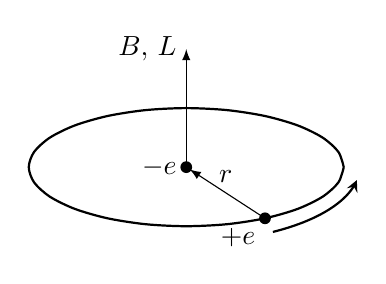
\begin{tikzpicture}[declare function={f(\x)=\ra*cos(\x) +\rb*sin(\x);}]
\pgfmathsetmacro{\ra}{2}
\pgfmathsetmacro{\rb}{0.75}
\pgfmathsetmacro{\rc}{\ra+0.2}
\pgfmathsetmacro{\rd}{\rb+0.2}
\draw[thick,domain=0:360]plot[smooth]({\ra*cos(\x)},{\rb*sin(\x)});
\draw [-latex] (0,0) node[left]{$-e$} node[fill=black, circle, inner sep=1.5pt]{} -- (0,1.5) node[left]{$\kvec{B}, \, \mat{L}$};
\draw [latex-,shorten <=1.5pt] (0,0) -- ({\ra*cos(300)},{\rb*sin(300)}) node[pos=0.5,above]{$r$} node[fill=black, circle, inner sep=1.5pt]{} node[below left]{$+e$};
\draw[-stealth,thick,domain=300:350]plot({\rc*cos(\x)},{\rd*sin(\x)});
\end{tikzpicture}
\caption{الیکٹران کے نقطہ نظر سے ہائیڈروجن جوہر۔}
\label{شکل_غیر_تابع_اضطراب_جوہر_الیکٹران_نقطہ_نظر}
\end{figure}

ہمیں پروٹان کا مقناطیسی میدان  اور الیکٹران کا جفت قطب معیار اثر \عددی{\kvec{\mu}} درکار ہوگا 

پروٹان کا مقناطیسی میدان ہم الیکٹران کی نقطہ نظر سے پروٹان کو استمراری دائری  رو (شکل \حوالہ{شکل_غیر_تابع_اضطراب_جوہر_الیکٹران_نقطہ_نظر})   تصور کرکے اس کے مقناطیسی میدان کو بایوٹ و سيوارٹ قانون سے حاصل کرتے ہیں 
\begin{align*} 
B = \frac{\mu_0 I}{2r}
\end{align*}
جس میں موثر رو \عددی{ I = e/T} ہے جہاں \عددی{ e} پروٹان کے بار کو اور \عددی{ T} دائرے پر ایک چکر کے دوری عرصہ کو ظاہر کرتا ہے اس کے برعکس مرکزہ کے ساکن  چھوکٹ میں الیکٹران کا مداری زاویائی معیار حرکت \عددی{
L = rmv = {2\pi m r ^2} /T
} ہوگا مزید \عددی{ \kvec{B}} اور \عددی{\mat{L}} دونوں کا رخ ایک   جیسا ہوگا شکل \حوالہ{شکل_غیر_تابع_اضطراب_جوہر_الیکٹران_نقطہ_نظر} میں اوپر جانب لہٰذا   درج ذیل لکھا جا سکتا ہے 
\begin{align}
\kvec{B} = \frac{1}{4 \pi \epsilon_0} \frac{e}{mc^2 r^3} \mat{L}
\end{align}
جہاں میں نے \عددی{
c = 1/\sqrt{\epsilon_0 \mu_0}
} استعمال کرکے \عددی{\mu_0} کی جگہ \عددی{\epsilon_0} استعمال کیا ہے 

الیکٹران کا مقناطیسی جفت قطب معیار اثر: ایک چکر کھاتے بار کا مقناطیسی جفت قطب معیار اثر اس کے چکر زاویائی معیار حرکت سے تعلق رکھتا ہے ان کے بیچ تناسبی جزو ضرب مسکن مقناطیسی مثبت ہوگا جس کا سامنا ہم حصہ 4.4.2 میں کر چکے ہیں آئیں اس مرتبہ  کلاسیکی برقی حرکیات استعمال کرتے ہوئے اسے اخذ کریں ایک ایسا بار \عددی{ q} جس کی لپائی  رداس \عددی{ r} کے چلا پر  کی گئی ہو اور جو محور کے گرد دوری عرصہ \عددی{ T} سے گھومتا ہو پر غور کریں(شکل  \حوالہ{شکل_غیر_تابع_اضطراب_چھلا_بار})۔   اس چھلے کے مقناطیسی جفت قطب معیار اثر کی تعریف رو \عددی{(q/T)} ضرب رقبہ \عددی{(\pi r^2)} ہے 
\begin{align*}
\mu = \frac{q \pi r^2}{T}
\end{align*}

\begin{figure}
\centering
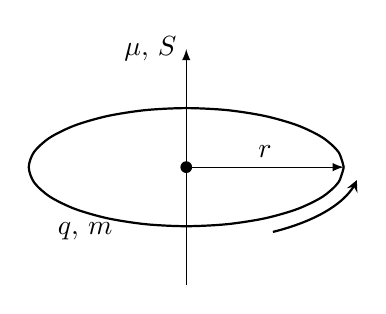
\begin{tikzpicture}[declare function={f(\x)=\ra*cos(\x) +\rb*sin(\x);}]
\pgfmathsetmacro{\ra}{2}
\pgfmathsetmacro{\rb}{0.75}
\pgfmathsetmacro{\rc}{\ra+0.2}
\pgfmathsetmacro{\rd}{\rb+0.2}
\draw[thick,domain=0:360]plot[smooth]({\ra*cos(\x)},{\rb*sin(\x)});
\draw [-latex] (0,-1.5) -- (0,1.5) node[left]{$\kvec{\mu}, \, \mat{S}$};
\draw [-latex] (0,0)node[circle,inner sep=1.5pt,fill=black]{} -- ({\ra*cos(0)},{\rb*sin(0)}) node[pos=0.5,above]{$r$};
\draw[-stealth,thick,domain=300:350]plot({\rc*cos(\x)},{\rd*sin(\x)});
\draw []  ({\ra*cos(230)},{\rb*sin(230)}) node[below]{$q,\, m$};
\end{tikzpicture}
\caption{بار کا چھلا جو اپنے محور کے گرد گھوم رہا ہے۔}
\label{شکل_غیر_تابع_اضطراب_چھلا_بار}
\end{figure}

اگر چھلا کی کمیت \عددی{ m} ہو جمودی معیار اثر \عددی{mr^2} ضرب زاویائی سمتی رفتار \عددی{(2 \pi/T)} اس کا زاویائی معیار حرکت ہوگا 
\begin{align*} 
S = \frac{2 \pi mr^2}{T}
\end{align*}
اس  تشکیل   کے لیے ظاہر ہے کہ مسکن مقناطیسی نسبت \عددی{
\mu /S = q/2m
} ہوگا دھیان رہے کہ یہ \عددی{ r} اور \عددی{ T} کا  تابع نہیں  ہے اگر میرے پاس کوئی زیادہ پیچیدہ شکل و صورت کا جسم ہوتا مثلاً  ایک  کرہ  صرف اتنا ضروری ہے کہ اپنے محور کے گرد گھومنے سے اس جسم کی شکل پیدا ہو میں اس کو باریک چھلوں میں ٹکڑے کر کے تمام  سے پیدا حصوں کا مجموعہ لے کر \عددی{\kvec{\mu}} اور \عددی{\mat{S}} کی قیمت معلوم کر پاتا جب تک کمیت اور بار کی تقسیم ایک جیسی ہو تاکہ بار اور کمیت کا نسبت یکساں ہو ہر  چھلے  کا اور لہٰذا   پوری جسم کا مسکن مقناطیسی نسبت ایک  جیسا ہوگا مزید \عددی{\kvec{\mu}} اور \عددی{\mat{S}} کے رخ ایک  جیسے یا اگر بار منفی ہو تو ایک دونوں کے مخالف ہونگے لہٰذا   درج ذیل ہوگا 
\begin{align*}
\kvec{\mu} = \big ( \frac{q}{2m} \big ) \mat{S}
\end{align*}
یہ خالصاً  کلاسیکی حساب ہے درحقیقت الیکٹران کا مقناطیسی معیار اثر اس کے کلاسیکی قیمت کا دگنا ہے 
\begin{align}
\kvec{\mu}_e = - \frac{e}{m} \mat{S}
\end{align}
ڈیراک   نے الیکٹران کی اضافیتی نظریہ میں اضافی جزو ضربی \عددی{2} کی وجہ پیش کی ہے

 ان تمام کو اکٹھے کرتے ہوئے درج ذیل حاصل ہوگا 
\begin{align*}
H = \big ( \frac{e^2}{4 \pi \epsilon_0} \big ) \frac{1}{m^2 c^2 r^3} \mat{S} \cdot \mat{L}
\end{align*}
اس حساب میں ایک  فریب سے کام لیا گیا ہے میں نے الیکٹران کے ساکن  چھوکٹ میں تجزیہ کیا جو ایک غیر جمودی نظام ہے چونکہ الیکٹران مرکزہ کے گرد گھومتا ہے لہٰذا   یہ اسراع  پذیر ہوگا اس حساب میں مجرد حرکیات تصحیح جسے طامس استقبالی حرکت کہتے ہیں شامل کرکے قبول کیا جا سکتا ہے جو حساب میں جزو ضربی \عددی{1/2} شامل کرتا ہے 
\begin{align}
H'_{so} = \big ( \frac{e^2}{8 \pi \epsilon_0} \big ) \frac{1}{m^2 c^2 r^3} \mat{S} \cdot \mat{L}
\end{align}
%=====================


یہ چکر و دائری  باہم عمل ہے۔ ماسوائے دو تصحیح (الیکٹران کی ترمیم شدہ مسکن مقناطیسی نسبت  اور طامس استقبالی حرکت جزو ضربی جو اتفاقاً ایک دوسرے کو کاٹتے  ہیں)  یہ وہی نتیجہ ہے جو آپ (بھولی بھالی)  کلاسیکی نمونہ سے حاصل کرتے۔ طبی طور پر یہ الیکٹران کے لمحاتی ساکن چھوکٹ  میں پروٹان کی مقناطیسی میدان میں، چکر کاٹتے الیکٹران کے مقناطیسی جفت قطب معیار اثر پر قوت مروڑ کی بدولت ہے۔

 اب کوانٹم میکانیات کی بات کرتے ہیں۔ چکر و دائری ربط کی صورت میں \عددی{ L} اور \عددی{ S} کے ساتھ ہیملٹنی غیر مقلوب ہو گا لہٰذا چکر اور دائری زاویائی معیار اثر علیحدہ علیحدہ   بقائی  نہیں رہتے ہیں سوال 6.16 دیکھیں البتہ \عددی{H'_{so}} مقلوب ہو گا \عددی{L^2}، \عددی{S^2} اور کل زاویائی معیار حرکت کے ساتھ۔
\begin{align}
\mat{J} \equiv \mat{L} + \mat{S}
\end{align}
 لہٰذا   یہ مقداریں   بقائی ی ہیں مساوات 3.71 دوسرے لفظوں میں \عددی{L_z} اور \عددی{S_z} کے امتیازی حالات نظریہ اضطراب میں استعمال کے لئے موزوں حالات نہیں ہیں جبکہ \عددی{L^2}، \عددی{S^2}، \عددی{J^2}، اور \عددی{J_z} کے امتیازی حالات موزوں حالات ہیں اب 
\begin{align*}
J^2 = (\mat{L} + \mat{S}) \cdot (\mat{L} + \mat{S}) = L^2 + S^2 + 2 \mat{L} \cdot \mat{S}
\end{align*}
کی بنا پر 
\begin{align}
\mat{L} \cdot \mat{S} = \frac{1}{2} (J^2 - L^2 - S^2)
\end{align}
ہوگا  لہٰذا   \عددی{
\mat{L} \cdot \mat{S}
} کے امتیازی اقدار درج ذیل ہونگے 
\begin{align*}
\frac{\hslash^2}{2} [j (j + 1) - l(l + 1) - s(s + 1)]
\end{align*}
یہاں یقیناً \عددی{S = 1/2} ہے مزید \عددی{1/r^3} کی توقعاتی قیمت سوال 6.35 (ج) دیکھیں درج ذیل ہے 
\begin{align}
\langle 1/r^3 \rangle = \frac{1}{l(l + 1/2) (l + 1) n^3 a^3} 
\end{align}
 لہٰذا   ہم درج ذیل اخذ کرتے ہیں 
\begin{align*}
E_{so}^1 = \langle H'_{so} \rangle = \frac{e^2}{8 \pi \epsilon_0} \frac{1}{m^2 c^2} \frac{(\hslash^2 /2) [j(j + 1) - l(l + 1) - 3/4]}{l(l + 1/2)(l + 1)n^3 a^3}
\end{align*} 
یا تمام کو \عددی{E_n} کی صورت میں لکھتے ہیں 
\begin{align}
E^1_{so} = \frac{(E_n)^2}{mc^2} \big \{ \frac{[j(j + 1) - l(l + 1) - 3/4]}{l(l + 1/2)(l + 1)} \big \}
\end{align}
یہ ایک حیرت کن بات ہے کہ بالکل مختلف طبیعی پہلوؤں کے باوجود اضافیتی تصحیح اور چکر و دائری بط ایک جتنا رتبہ \عددی{(E_n^2 / mc^2)} رکھتے ہیں ان دونوں کو جمع کرکے ہمیں مکمل مہین ساخت کا کلیہ سوال 6.17 دیکھیں حاصل ہوتا ہے 
\begin{align}
E_{fs}^1 = \frac{(E_n)^2}{2mc^2} \big ( 3 - \frac{4n}{j + 1/2} \big )
\end{align}
اس کو کلیہ بوہر کے ساتھ چھوڑ کر ہم ہائیڈروجن کی توانائی کی سطحوں کا عظیم نتیجہ حاصل کرتے ہیں جس میں مہین ساخت شامل ہے 
\begin{align}
E_{nj} = - \frac{\SI{13.6}{\electronvolt}}{n^2} \big [ 1 + \frac{\alpha^2}{n^2} \big ( \frac{n}{j + 1/2} - \frac{3}{2} \big ) \big ]
\end{align}
مہین ساخت \عددی{l} میں انحطاط کو توڑتا ہے یعنی کسی ایک \عددی{ n} کیلئے \عددی{l} کی مختلف اجازتی قیمتیں ایک  جیسی توانائی کے حامل نہیں ہونگی تاہم اب بھی یہ \عددی{ j} میں انحطاط  برقرار رکھتا ہے شکل 6.9  دیکھیں دائری و چکر زاویائی معیار حرکت  کے \عددی{ z} جزو امتیازی اقدار \عددی{m_l} اور \عددی{m_s} اب موزوں کوانٹم اعداد نہیں ہونگے۔ ان مقداروں کی مختلف قیمتوں والے حالات کے خطی جوڑ ساکن حالات ہوں گے۔ ‏موزوں کوانٹم اعداد \عددی{n}، \عددی{l}، \عددی{s}، \عددی{j}، اور \عددی{m_j} ہونگے 
\ابتدا{سوال}
درج ذیل مقلب کی قیمتیں تلاش کریں
 ( الف) \عددی{
[\mat{L} \cdot \mat{S}, \mat{L}]
}، ( ب) \عددی{
[\mat{L} \cdot \mat{S}, \mat{S}]
}، ( ج) \عددی{
[\mat{L} \cdot \mat{S}, \mat{J}]
}، ( د) \عددی{
[\mat{L} \cdot \mat{S}, L^2]
}، ( ه) \عددی{
[\mat{L} \cdot \mat{S}, S^2]
}، ( و) \عددی{
[\mat{L} \cdot \mat{S}, J^2]
}؛ اشارہ: \عددی{\mat{L}} اور \عددی{\mat{S}} زاویائی معیار حرکت کے بنیادی مقلبیت رشتوں مساوات 4.99 اور 4.134 کو مطمئن کرتے ہیں تاہم یہ ایک دوسرے کے ساتھ غیر مقلوب ہیں۔ 
\انتہا{سوال}
\ابتدا{سوال}
اضافیتی تصحیح مساوات 6.57 اور چکر دائری ربط مساوات 6.65 سے مہین ساخت کلیہ مساوات 6.66 اخذ  کریں اشارہ: دھیان رہے کہ \عددی{
j = l \pm 1/2 
} ہے مثبت علامت اور منفی علامت کو باری باری لے کر دیکھیں آپ دیکھیں گے کہ دونوں صورتوں میں آخری نتیجہ ایک  دوسروں  جیسا ہوگا 
\انتہا{سوال} 
\ابتدا{سوال}
 ہائیڈروجن کے موئی   طیف  کی  سرخ  بالمر لکیر نمایاں ہے جو \عددی{n = 3} سے \عددی{n = 2} میں منتقلی سے پیدا ہوتی ہے اس طیفی  لکیر کا طول موج اور تعدد بوہر نظریہ سے تعین کریں مہین ساخت اس لکیر کو قریب قریب کئی لکیروں میں تقسیم کرتا ہے اب سوال یہ پیدا ہوتا ہے: لکیروں کی تعداد کیا ہو گی  اور ان  کے بیچ فاصلہ کتنا ہو گا اشارہ: پہلے قدم میں معلوم کریں کہ \عددی{n = 2} سطح کتنی ذیلی سطحوں میں تقسیم ہوگا اور ہر ایک کے لیے \عددی{
\si{\electronvolt}
} میں \عددی{E_{fs}^1} تلاش کریں یہی کچھ \عددی{n = 3} کے لیے کریں سطح توانائی کے شکل کا خاکہ بنا کر \عددی{n = 3} سے \عددی{n = 2} تک تمام   ممکنہ منتقلی دکھائیں نوریہ کی صورت میں توانائی کا اخراج    \عددی{(E_3 - E_2) + \Delta E} ہوگا جہاں پہلا جزو سب میں مشترک  جبکہ مہین ساخت کی      بدولت  \عددی{\Delta E} کی قیمت  ایک منتقلی سے دوسرے منتقلی  بدلے گی۔        ہر منتقلی کے لئے \عددی{\Delta E} کو \عددی{\si{\electronvolt}} میں تلاش         کریں آخر میں انہیں نوریہ تعدد میں تبدیل کرکے  ساتھ ساتھ طیفی لکیروں کے بیچ فاصلہ \عددی{\si{\hertz}} کی صورت   میں تعین کریں یہ غیر مضطرب لکیر اور ہر ایک طیفی لکیر کے بیچ تعددی فاصلہ نہیں ہوگا جو یقیناً قابل مشاہدہ نہیں ہے بلکہ یہ ہر لکیر اور اگلے لکیر کے بیچ تعددی فاصلہ ہوگا آپ کا جواب درج ذیل روپ میں ہونا چاہیے  سرخ  بالمر لکیر \عددی{(؟؟؟)} لکیروں میں تقسیم ہوتا ہے بڑھتے تعدد کے لحاظ سے یہ \عددی{(1)} \عددی{j = (???)} سے \عددی{j = (???)}، \عددی{2} \عددی{j = (???)} سے \عددی{j = (???)}، \عددی{\dotsc} ہونگے لکیر \عددی{1} اور لکیر \عددی{2} کے بیچ  تعددی فاصلہ \عددی{(???)} \عددی{\si{\hertz}} ہے لکیر \عددی{2} اور لکیر \عددی{3} کے بیچ فاصلہ \عددی{???} \عددی{\si{\hertz}} ہے \عددی{\dotsc} 
\انتہا{سوال}
\ابتدا{سوال}
نظریہ اضافت استعمال کیے بغیر ڈیراک مساوات سے ہائیڈروجن کی مہین ساخت کا ٹھیک ٹھیک کلیہ درج ذیل حاصل ہوتا ہے 
\begin{align*}
E_{nj} = mc^2 \big \{ \big [ 1 + \big ( \frac{\alpha}{n - (j + 1/2 ) + \sqrt{(j +1/2)^2 - \alpha^2}} \big )^2 \big ]^{- 1/2} -1 \big \}
\end{align*}
یہ ذہن میں رکھتے ہوئے کہ \عددی{
\alpha \ll 1
} ہے اس کو \عددی{a^4} رتبہ تک پھیلا کر دکھائیں کہ آپ مساوات 6.67 دوبارہ حاصل کرتے ہیں 
\انتہا{سوال} 
%===========================
%section 6.4 Zeeman effect
\حصہ{زیمان اثر} 
ایک جوہر کو یکساں بیرونی مقناطیسی میدان \عددی{
\kvec{B}_{ext}
} میں رکھنے سے اس کی توانائی کی سطحوں  میں تبدیلی پیدا ہوتی ہے اس مظہر کو زیمان اثر کہتے ہیں واحد ایک الیکٹران کے لیے اضطراب درج ذیل ہوگا 
\begin{align} 
H'_z = - (\mu_1 + \mu_2) \cdot \kvec{B}_{est}
\end{align}
جہاں 
\begin{align}
\mu_s = - \frac{e}{m} \mat{S}
\end{align}
الیکٹران چکر کے ساتھ وابستہ مقناطیسی جفت کتب معیار اثر اور 
\begin{align} 
\mu_1 = - \frac{e}{2m} \mat{L}
\end{align}
مداری حرکت کے ساتھ وابستہ جفت کتب معیار اثر ہے یوں  درج ذیل ہوگا 
\begin{align}
H'z = \frac{e}{2m} (\mat{L} + 2 \mat{S}) \cdot \kvec{B}_{est}
\end{align}
زیمان تقسیم کی فطرت فیصلہ کن حد تک اندرونی میدان مساوات 6.59 جو چکر مدار ربط پیدا کرتا ہے کے لحاظ سے بیرونی میدان کی طاقت پر منحصر ہوگا اگر  \عددی{
B_{ext} \ll B_{int}
} ہو تب مہین ساخت غالب ہوگا اور \عددی{H'} کو ایک چھوٹی اضطراب تصور کیا جا سکتا ہے جبکہ \عددی{
B_{ext} \gg B_{int}
} کی صورت میں زیمان  اثر غالب ہوگا اور مہین ساخت خود اضطراب تصور کی جائے گی ان دو خطوں کے بیچ جہاں دونوں میدان  مقلوب  ہے ہمیں انحطاطی نظریہ اضطراب کی پوری قوت درکار ہوگی اور ہم پر  لازم ہوگا کہ ہم ہیملٹنی کی متعلقہ حصے کو ہاتھ سے وتری بنائیں درج ذیل حصوں میں ہم ان تین صورتوں پر ہائیڈروجن کے لیے غور کریں گے 
\ابتدا{سوال} 
مساوات 6.59 استعمال کرتے ہوئے ہائیڈروجن کی اندرونی میدان کی اندازاً  قیمت تلاش کرکے بتائیں  کہ  طاقتور اور کمزور زیمان میدان کتنا ہوگا 
\انتہا{سوال} 
\جزوحصہ{کمزور میدان زیمان اثر}
اگر \عددی{
B_{ext} \ll B_{int}
} ہو تب مہین ساخت مساوات 6.67 غالب ہوگی اور موزوں کوانٹم اعداد \عددی{n}، \عددی{l}، \عددی{j}، اور \عددی{m_j} ہونگے تاہم چکر و مدار ربط کی موجودگی میں \عددی{\mat{L}} اور \عددی{\mat{S}} علیحدہ علیحدہ بقائی نہیں ہونگے لہٰذا \عددی{m_l} اور \عددی{m_s} موزوں کوانٹم اعداد نہیں ہونگے رتبہ اول نظریہ اضطراب میں توانائی میں زیمان تصحیح درج ذیل ہوگی 
\begin{align}
H_Z^1 = \langle nljm_j | H'_Z | nljm_j \rangle = \frac{e}{2m} \kvec{B}_ext \cdot \langle \mat{L} + 2 \mat{S} \rangle 
\end{align} 
اب \عددی{
\mat{L} + 2 \mat{S} = \mat{J} + \mat{S}
} ہوگا بدقسمتی سے ہمیں \عددی{\mat{S}} کی توقعاتی قیمت فوری طور پر معلوم نہیں ہے لیکن ہم درج ذیل طریقہ سے اسے جان سکتے ہیں کل زاویائی معیار حرکت \عددی{
\mat{J} = \mat{L} + \mat{S}
} ایک مستقل ہے (شکل  \حوالہ{شکل_غیر_تابع_چکرومدار_غیر_بقائی})۔  اس مقررہ سمتیہ کے گرد \عددی{\mat{L}} اور \عددی{\mat{S}} تیزی سے استقبالی حرکت کرتے ہیں بالخصوص \عددی{\mat{J}} پر \عددی{\mat{S}} کی قائمہ تظلیل \عددی{\mat{S}} کی وقتی اوسط قیمت ہوگا 
\begin{align}
\mat{S}_{\text{\RL{اوسط}}}= \frac{(\mat{S} \cdot \mat{J})}{j^2} \mat{J} 
\end{align}
لیکن  \عددی{
\mat{L} = \mat{J} - \mat{S}
} ہے لہٰذا \عددی{
L^2 = J^2 + S^2 - 2 \mat{J} \cdot \mat{S}
} ہوگا لہٰذا 
\begin{align}
\mat{S} \cdot \mat{J} = \frac{1}{2} (J^2 + S^2 - L^2) = \frac{\hslash^2}{2} [j(j + 1) + s(s + 1) - l(l + 1)]
\end{align}
جس سے درج ذیل حاصل ہوتا ہے 
\begin{align}
\langle \mat{L} + 2 \mat{S} \rangle = \langle \big ( 1 + \frac{\mat{S} \cdot \mat{J}}{J^2} \big ) \mat{J} \rangle = \big [ 1 + \frac{j (j + 1) - l (l + 1) + 3/4}{2 j (j + 1)} \big ] \langle \mat{J} \rangle
\end{align}
چوکور  قوسین   میں بند رکن کو لنڈے \عددی{ g} جزو ضرب کہتے ہیں جس کو \عددی{g_j} سے ظاہر کیا جاتا ہے ہم محور \عددی{z} کو \عددی{
\kvec{B}_{ext}
} کے ساتھ ساتھ رکھ سکتے ہیں تب درج ذیل ہوگا 
\begin{align}
E_Z^1 = \mu_B g_J B_{ext} m_j
\end{align}
جہاں 
\begin{align}
\mu_B \equiv \frac{e \hslash}{2m} = \SI{5.788e-5}{\electronvolt\per T}
\end{align}
بوہر مقناطیسہ کہلاتا ہے مہین ساخت کا حصہ مساوات 6.67 اور زیمان کا حصہ مساوات 6.76 کا مجموعہ کل توانائی دے گا مثال کے طور پر زمینی حال \عددی{n = 1}، \عددی{l = 0}، \عددی{j = 1/2} لہٰذا \عددی{g_j = 2} دو سطحوں میں  بٹ  جائے گا 
\begin{align}
\SI{- 13.6}{\electronvolt} (1 + \alpha^2 /4) \pm \mu_B B_{ext}
\end{align}
جہاں \عددی{m_j = 1/2} کے لیے مثبت علامت اور \عددی{m_j = -1/2} کے لیے منفی علامت استعمال ہوگی ان توانائیوں کو \عددی{B_{ext}} کے تفاعل کے طور پر شکل 6.11 ترسیم کیا گیا ہے۔
\begin{figure}
\centering
\pgfmathsetmacro{\ra}{2}
\pgfmathsetmacro{\rb}{0.75}
\begin{tikzpicture}[declare function={f(\x)=\ra*cos(\x); g(\x)=\rb*sin(\x);}]
\draw[rotate around={-45:(0,0)}, domain=0:360] plot[smooth] ({f(\x)},{g(\x)});
\draw[rotate around={-45:(0,0)}, -stealth](0,-3) node[fill=black,circle,inner sep=1.5pt]{} -- (0,0) node[pos=0.5, above left] {$\mat{J}$} node[fill=black,circle,inner sep=1.5pt]{} -- (0,2);
\draw[rotate around={-45:(0,0)}, -stealth] (0,-3) -- ({f(330)},{g(330)}) node[pos=0.5, below right]{$\mat{L}$};
\draw[rotate around={-45:(0,0)}, -stealth] ({f(330)},{g(330)}) -- (0,2) node[pos=0.75, above right]{$\mat{S}$};
\end{tikzpicture}
\caption{چکر و مدار ارتباط کی عدم موجودگی میں \عددی{\mat{L}} اور \عددی{\mat{S}} علیحدہ علیحدہ  بقائی نہیں ہوں گے؛ یہ اٹل  کل  زاویائی معیار  حرکت \عددی{\mat{J}}  کے گرد استقبالی حرکت کرتے ہیں۔} 
\label{شکل_غیر_تابع_چکرومدار_غیر_بقائی}
\end{figure}

 
\ابتدا{سوال} 
آٹھ عدد \عددی{n = 2} حالات \عددی{| 2ljm_j \rangle} پر غور کریں کمزور میدان زیمان بٹنے  کی صورت میں ہر حال کی توانائی تلاش کرکے شکل  \حوالہ{شکل_غیر_تابع_اضطراب_زیمان_بٹوارا_کمزور_میدان}  کی طرز کا خاکہ بنا کر دکھائیں \عددی{B_{ext}} بڑھانے سے توانائیاں کس طرح ارتقا کرتی ہے ہر خط کو نام دے کر اس کی ڈھلوان دکھائیں ۔
\begin{figure}
\centering
\begin{tikzpicture}
\pgfmathsetmacro{\a}{40}
\pgfmathsetmacro{\b}{180-\a}
\pgfmathsetmacro{\c}{0.4}
\draw[thick] (0,0) node[circle, fill=black, inner sep=1.5pt]{} --++ (-45:2.5) node[right]{$m_j = -1/2$};
\draw[thick] (0,0)node[left]{$-13.6(1+\alpha^2/4)\,\si{\electronvolt}$} --++ (45:2.5) node[right]{$m_j = 1/2$};
\draw(0,-1.5) -- (0,2) to [out=-\a, in =-\b] ++(\c,0) (0,2) to [out=\b, in =\a] ++(-\c,0) (0,2.15) to [out=-\a, in =-\b] ++(\c,0) (0,2.15) to [out=\b, in =\a] ++(-\c,0) ;
\draw[-latex](0,2.15) --++ (0,1) node[left]{$E$};
\draw[-latex](-0.5,2.5) --++ (4,0) node[above]{$\mu_B B_{\text{بیرونی}}$};
\end{tikzpicture}
\caption{ہائیڈروجن کے زمینی حال کی کمزور میدانی زیمان بٹوارا؛ بالائی  لکیر  \عددی{(m_j=1/2)} کی ڈھلوان \عددی{1} ہے؛ نچلی لکیر \عددی{(m_j=-1/2)} کی ڈھلوان \عددی{-1} ہے۔}
\label{شکل_غیر_تابع_اضطراب_زیمان_بٹوارا_کمزور_میدان}
\end{figure}


\انتہا{سوال} 

\جزوحصہ{طاقتور میدان زیمان اثر}
اگر \عددی{
B_{ext} \gg B_{int} 
} ہو تب زیمان  اثر غالب ہوگا میدان \عددی{B_{ext}} کو \عددی{ z} محور پر رکھ کر موزوں کوانٹم اعداد \عددی{n}، \عددی{l}، \عددی{m_l}، اور \عددی{m_s} ہونگے جبکہ \عددی{ j} اور \عددی{m_j} نہیں ہونگے چونکہ بیرونی قوت مروڑ کی صورت میں کل ضیائی معیار حرکت بقائی  نہیں ہوگا جبکہ \عددی{L_z} اور \عددی{S_z} ہونگے زیمان ہیملٹنی 
\begin{align*}
H'_Z = \frac{e}{2m} B_{ext} (L_z + 2S_z)
\end{align*}
جبکہ غیر مضطرب توانائی درج ذیل ہونگی 
\begin{align}
E_{nmlms} = - \frac{\SI{13.6}{electronvolt}}{n^2} + \mu_B B_{ext} (m_l + 2m_s)
\end{align}
مہین ساخت کو مکمل نظرانداز کرتے ہوئے یہی جواب ہوگا تاہم اس سے بہتر کر سکتے ہیں رتبہ اول نظریہ اضطراب میں ان سطحوں کی مہین ساخت تصحیح درج ذیل ہوگی 
\begin{align}
E_{fs}^1 = \langle nlm_l m_s | (H'_r + H'_so) | \rangle nlm_l m_s \rangle
\end{align}
اضافیتی قصہ وہی ہوگا جو پہلے تھا مساوات 6.57 چکر و مدار جزو مساوات 6.61 کے لیے ہمیں درج ذیل درکار ہوگا 
\begin{align}
\langle \mat{S} \cdot \mat{L} \rangle = \langle S_x \rangle \langle L_x \rangle + \langle S_y \rangle \langle L_y \rangle + \langle S_z \rangle \langle L_y \rangle = \hslash^2 m_l m_s
\end{align}
دھیان رہے کہ \عددی{S_z} اور \عددی{L_z} کہ امتیازی تفاعلات کے لیے \عددی{
\langle S_x \rangle = \langle S_y \rangle = \langle L_x \rangle = \langle Ly \rangle=0
} ہوگا ان تمام کو اکٹھے کرکے سوال 6.22 ہم درج ذیل اخذ کرتے ہیں 
\begin{align}
E_{fs}^1 = \frac{\SI{13.6}{\electronvolt}}{n^3} \alpha^2 \big \{ \frac{3}{4n} - \big [ \frac{l(l + 1) - m_l m_s}{l(l + 1/2)(l + 1)} \big ] \}
\end{align}
 چوکور  قوسین   کا جزو \عددی{l = 0} کے لئے غیر تعین ہوگا یہاں اس کی درست قیمت ایک ہے سوال 6.24 دیکھیں زیمان حصہ مساوات 6.79 اور مہین ساخت حصہ مساوات 6.82 کا مجموعہ کل توانائی دے گا 
\ابتدا{سوال}
مساوات 6.80 سے آغاز کر کے مساوات 6.57، 6.61، 6.64، اور 6.81 استعمال کرتے ہوئے مساوات 6.82 اخذ کریں 
\انتہا{سوال}
\ابتدا{سوال}
آٹھ عدد \عددی{n = 2} حالات  \عددی{
| 2l m_j m_s \rangle
} پر غور کریں طاقتور میدان زیمان بانٹ کی صورت میں ہر حال کی توانائی تلاش کرے اپنے جواب کو بوہر توانائی  \عددی{l^2} کے راست متناسب مہین ساخت اور  \عددی{\mu_B B_{ext}} کے براہ راست متناسب زیمان حصہ کہ مجموعہ کی صورت میں لکھیں مہین  ساخت کو مکمل طور پر نظر انداز کرتے ہوئے منفرد سطحوں کی تعداد کتنی ہوگی اور ان کے انحطاط کیا ہونگے 
\انتہا{سوال}
\ابتدا{سوال}
اگر \عددی{l = 0} ہو تب \عددی{j = s}، \عددی{m_j = m_s} ہوگا لہٰذا کمزور اور طاقتور میدانوں کے لیے موزوں حالات \عددی{
(|nm_s \rangle)
} ایک  جیسے ہوں گے مساوات 6.72 سے \عددی{E_Z^1} اور مساوات 6.67 سے مہین ساخت توانائیاں تعین کر کے میدان کی طاقت سے قطع نظر \عددی{l = 0} کیلئے زیمان اثر کا عمومی نتیجہ لکھیں دکھائیں کے درمیانی چوکور قوسین   رکن کی قیمت ایک لیتے ہوئے طاقتور میدان کلیہ مساوات 6.82 یہی نتیجہ دے گا 
\انتہا{سوال}
%============================

\جزوحصہ{درمیانی طاقت میدان زیمان اثر} 
درمیانی طاقت میدان کی صورت میں نہ \عددی{H'_Z} اور نہ ہی \عددی{H'_{fs}} غالب ہوگا لہذا ہمیں دونوں کو ایک نظر سے دیکھ کر بوہر ہیملٹنی مساوات 6.42 کے اضطراب تصور کرنا ہوگا 
\begin{align}
H' = H'_Z + H'_{fs}
\end{align}
میں \عددی{n = 2} صورت پر اپنی توجہ محدود کرتے ہوئے وہ حالات جن کی وصف \عددی{l}، \عددی{j}، اور \عددی{m_j} بیان کرتی ہے کو انحطاطی نظریہ اضطراب کا اساس لیتا ہوں كليبش گورڈن عددی سر سوال 4.51 یا جدول 4.8 استعمال کرتے ہوئے \عددی{
| j m_j \rangle 
} کو \عددی{
| lm_l \rangle | sm_s \rangle
} کا خطی جوڑ لکھ کر درج ذیل ہوگا 
\begin{align*}
l &= 0
\begin{cases}
\psi_1 \equiv | \frac{1}{2} \frac{1}{2} \rangle = | 00 \rangle | \frac{1}{2} \frac{1}{2} \rangle \\
\psi_2 \equiv | \frac{1}{2} \frac{-1}{2} \rangle = | 00 \rangle | \frac{1}{2} \frac{-1}{2} \rangle
\end{cases} \\
l &= 1
\begin{cases}
\psi_3 \equiv | \frac{3}{2} \frac{3}{2} \rangle = | 11 \rangle | \frac{1}{2} \frac{1}{2} \rangle \\
\psi_4 \equiv | \frac{3}{2} \frac{-3}{2} \rangle = | 1 - 1 \rangle | \frac{1}{2} \frac{-1}{2} \rangle \\
\psi_5 \equiv | \frac{3}{2} \frac{1}{2} \rangle = \sqrt{2/3}| 10 \rangle | \frac{1}{2} \frac{1}{2} \rangle + \sqrt{1/3} | 11 \rangle \frac{1}{2} \frac{-1}{2} \rangle \\
\psi_6 \equiv | \frac{1}{2} \frac{1}{2} \rangle = - \sqrt{1/3} | 10 \rangle | \frac{1}{2} \frac{1}{2} \rangle + \sqrt{2/3} | 11 \rangle \frac{1}{2} \frac{-1}{2} \rangle \\
\psi_7 \equiv | \frac{3}{2} \frac{-1}{2} \rangle = \sqrt{1/3} | 1 - 1 \rangle | \frac{1}{2} \frac{1}{2} \rangle + \sqrt{2/3} | 10 \rangle \frac{1}{2} \frac{-1}{2} \rangle \\
\psi_8 \equiv | \frac{1}{2} \frac{-1}{2} \rangle = - \sqrt{2/3} | 1 - 1 \rangle | \frac{1}{2} \frac{1}{2} \rangle + \sqrt{1/3} | 10 \rangle \frac{1}{2} \frac{-1}{2} \rangle
\end{cases}
\end{align*}

اس اساس میں \عددی{H'_{fs}} کے تمام غیر صفر  قالبی ارکان جنہیں مساوات 6.66 دیتی ہے وتر پر پائے جاتے ہیں \عددی{H'_Z} کے چار غیر وتری ارکان پائے جاتے ہیں اور \عددی{
- \mat{W}
} کا مکمل قالب سوال 6.25 دیکھیں درج ذیل ہوگا  
\begin{align*}
5 \gamma - \beta & 0 & 0 & 0 & 0 & 0 & 0 & 0 \\
0 & 5 \gamma + \beta & 0 & 0 & 0 & 0 & 0 & 0 \\
0 & 0 & \gamma - 2 \beta & 0 & 0 & 0 & 0 & 0 \\
0 & 0 & 0 &  \gamma + 2 \beta & 0 & 0 & 0 & 0 \\
0 & 0 & 0 & 0 & \gamma - \tfrac{2}{3} \beta & \tfrac{\sqrt{2}}{3} \beta & 0 & 0 \\
0 & 0 & 0 & 0 & \tfrac{\sqrt{2}}{3} \beta & 5 \gamma - \tfrac{1}{3} \beta & 0 & 0 \\
0 & 0 & 0 & 0 & 0 & 0 & \gamma + \tfrac{2}{3} \beta & \tfrac{\sqrt{2}}{3} \beta \\
0 & 0 & 0 & 0 & 0 & 0 & \tfrac{\sqrt{2}}{3} \beta & 5 \gamma + \tfrac{1}{3} \beta 
\end{align*}
جہاں درج ذیل ہوںگے 
\begin{align*}
\gamma \equiv (\alpha /8)^2 \SI{13.6}{\electronvolt} \quad \text{\RL{اور}} \quad \beta \equiv \mu_B \kvec{B}_{ext}
\end{align*}
ابتدائی چار امتیازی اقدار پہلے سے وتر پر دکھائے گئے ہیں اب صرف دو \عددی{2 \times 2} ڈبوں کی امتیازی اقدار تلاش کرنا باقی ہے ان میں سے پہلی کی امتیازی مساوات درج ذیل ہے 
\begin{align*}
\lambda^2 - \lambda (6 \gamma - \beta) + \big ( 5 \gamma^2 - \frac{11}{3} \gamma \beta \big ) = 0
\end{align*}
جس سے دو درجی کلیہ درج ذیل امتیازی اقدار دے گا 
\begin{align}
\lambda_{\pm} = - 3 \gamma + (\beta /2) \pm \sqrt{4 \gamma^2 + (2/3) \gamma \beta + (\beta^2 /4)}
\end{align}
دوسرے ڈبے کی امتیازی اقدار یہی مساوات دے گی لیکن اس میں \عددی{\beta} کی علامت الٹ ہوگی ان آٹھ توانائیوں کو جدول 6.2 میں پیش کیا گیا ہے اور
 شکل  \حوالہ{شکل_غیر_تابع_اضطراب_کمزور_درمیانہ_طاقتور}  میں \عددی{B_{ext}} کے لحاظ سے ترسیم کیا گیا ہے صفر میدان حد \عددی{\beta = 0} میں یہ مہین ساخت قیمتیں دیتی ہیں کمزور میدان \عددی{
\beta \ll \gamma
} کی صورت میں یہ سوال 6.21 میں حاصل نتائج دیتی ہے طاقتور میدان  \عددی{\beta \gg \gamma} کی صورت میں سوال 6.23 کے نتائج حاصل ہونگے دھیان رہے جیسا سوال 6.23 میں پیشگوئی کی گئی تھی کہ بہت زیادہ طاقتور میدانوں میں یہ پانچ منفرد توانائیوں کی سطحوں پر مرکوز ہوں گے ۔
\begin{figure}
\centering
\begin{tikzpicture}
\draw[-stealth] (0,0) -- (5.5,0) node[below]{$\mu_B B_{\text{بیرونی}}$};
\draw[-stealth] (0,0) -- (0,5.5) node[left]{$E$};
\draw[](0,2.5) node[left]{$0$} --++ (0.2,0);
\draw[thick](0,2.6) -- (5,0.2);
\draw[thick](0,2.6) to [out=-10,in=175] (5,2.0);
\draw[thick](0,2.6) to [out=5, in=-163] (5,3.7);
\draw[thick](0,2.6) -- (5,5);
\draw[thick, dashed](0,2.1) -- (5,0.5);
\draw[thick, dashed](0,2.1) -- (5,3.5);
\draw[thick](0,2.1) to [out=-5, in=160] (5,0.7);
\draw[thick](0,2.1) to [out=3, in=175] (5,1.8);
\draw[-stealth](0.25,5.25) -- (4.75,5.25) node[pos=0.1,fill=white]{کمزور} node[pos=0.4,fill=white]{درمیانہ} node[pos=0.75,fill=white]{طاقتور};
\end{tikzpicture}
\caption{کمزور، درمیانہ اور طاقتور میدان میں ہائیڈروجن کے  \عددی{n=2} حال کا  زیمان بٹوارا۔}
\label{شکل_غیر_تابع_اضطراب_کمزور_درمیانہ_طاقتور}
\end{figure}


\ابتدا{سوال}
قالبی ارکان \عددی{H_Z'} اور \عددی{H'_{fs}} دریافت کر کے \عددی{n=2} کے لئے متن  میں دیا گیا قالب \عددی{W} مرتب کریں۔
\انتہا{سوال}
\ابتدا{سوال} 
ہائیڈروجن کے \عددی{n = 3} حالات کے لیے کمزور، طاقتور اور درمیانی میدان خطوں کے لیے زيمان اثر کا تجزیہ کریں جدول 6.2 کی طرز پر توانائیوں کا جدول تیار کرکے انہیں بیرونی میدان کے تفاعل کے طور پر ترسیم کریں جیسا شکل 6.12 میں کیا گیا تصدیق کیجئے گا کہ درمیانے میدان کے نتائج دو تحدیدی صورتوں میں تحفیف ہو کر درست قیمتی دیتی ہے  
\انتہا{سوال}

%===================
\جزوحصہ{نہایت مہین بٹوارہ}
پروٹان خود ایک مقناطیسی جفت کتب  ہے اگرچہ نسب نما میں کمیت کی بنا پر اس کا جفت کتب معیار اثر الیکٹران کے جفت کتب معیار اثر سے بہت کم ہوگا مساوات 6.60 
\begin{align}
\kvec{\mu}_p = \frac{g_p e}{2 m_p} \mat{S}_p, \quad \kvec{\mu}_e = - \frac{e}{m_e} \mat{S}_e
\end{align}
پروٹان ایک مخلوط ساخت کا ذرہ ہے جو تین کوارکوں پر مشتمل ہے لہذا اس کا مسکن مقناطیسی نسبت الیکٹران کی مسکن مقناطیسی نسبت کی طرح سادہ نہیں ہوگا جس کی بنا پر  صريحى \عددی{g} جذب ضربی \عددی{g_p} لکھا گیا ہے جس کی پیمائشی قیمت 5.59 ہے جو الیکٹران کی قیمت دو سے مختلف ہے کلاسیکی برقی حرکیات کے تحت جفت کتب  \عددی{\mu} درج ذیل مقناطیسی میدان پیدا کرتا ہے 
\begin{align}
\kvec{B} = \frac{\mu_0}{4 \pi r^3} [3 (\kvec{\mu} \cdot \kvecsub{a}{r}) \kvecsub{a}{r} - \kvec{\mu}] + \frac{2 \mu_0}{3} \kvec{\mu} \delta^3 (\kvec{r})
\end{align}
یو پروٹان کے مقناطیسی جفت کتب معیار اثر سے پیدا مقناطیسی میدان میں الیکٹران کا ہیملٹنی درج ذیل ہوگا مساوات 6.58 
\begin{align}
H'_{hf} = \frac{\mu_0 g_p e^2}{8 \pi m_p m_e} \frac{[3(\mat{S}_p \cdot \kvecsub{a}{r})(\mat{S}_e \cdot \kvecsub{a}{r}) - \mat{S}_p \cdot \mat{S}_e]}{r^3} + \frac{\mu_0 g_p e^2}{3m_p m_e} \mat{S}_p \cdot \mat{S}_e \delta^3 ((\kvec{r}))
\end{align}
نظریہ اضطراب کے تحت توانائی کی اول رتبی تخفیف مساوات 6.9 اس طرح بھی ہيملٹنی کی توقعاتی قیمت ہوگی 
\begin{align}
E_{hf}^1 = \frac{\mu_0 g_p e^2}{8 \pi m_p m_e} \langle \frac{3(\mat{S}_p \cdot \kvecsub{a}{r})(\mat{S}_e \cdot \kvecsub{a}{r} - \mat{S}_p \cdot \mat{S}_e)}{r^3} \rangle + \frac{\mu _0 g_p e^2}{3 m_p m_e} \langle \mat{S}_p \cdot \mat{S}_e \rangle |\psi (0)|^2
\end{align}
زمینی ہال میں یا کسی دوسری ایسے حال میں جس میں \عددی{l = 0} ہو تفاعل موج کروی تشاکلی ہوگا لہذا اول توقعاتی قیمت صفر ہوگی سوال 6.27 دیکھیں ساتھ ہی مساوات 4.80 کے تحت \عددی{
|\psi_{100} (0)|^2 = 1/(\pi a^3)
} ہوگا لہذا زمینی ہال میں درج ذیل ہوگا 
\begin{align}
E_{hf}^1 = \frac{\mu_0 g_p e^2}{3 \pi m_p m_e a^3} \langle \mat{S}_p \cdot \mat{S}_e \rangle
\end{align}
چونکہ اس میں دو چکروں کے بیچ ضرب نقطہ پایا جاتا ہے لہذا اس کو چکر چکر ربط کہتے ہیں جیسا چکر مدار ربط میں \عددی{
\mat{S} \cdot \mat{L}
} پایا جاتا ہے چکر چکر ربط کی موجودگی میں انفرادی چکر زاویائی معیار اثر بقائی نہیں رہتے ہیں موزوں حالات کل چکر کے امتیازی سمتیات ہونگے 
\begin{align}
\mat{S} \equiv \mat{S}_e + \mat{S}_p
\end{align}
پہلے کی طرح ہم اس کا مربع لے کر درج ذیل حاصل کرتے ہیں 
\begin{align}
\mat{S}_p \cdot \mat{S}_e = \frac{1}{2} (S^2 - S_e^2 - S_p^2)
\end{align}
اب الیکٹران اور پروٹون دونوں کا چکر ایک بٹا دو ہے لہذا \عددی{
S_e^2 = S_p^2 = (3/4) \hslash^2
} ہوگا سہ تا حال تمام چکر متوازی میں کل چکر ایک ہوگا جس کے تحت \عددی{
S^2 = 2 \hslash^2
} ہوگا یکتا حال میں کل چکر صفر لہذا \عددی{S^2 = 0} ہوگا یوں درج ذیل ہوگا 
\begin{align}
E_{hf}^1 = \frac{4g_p \hslash^4}{3m_p m_e^2 c^2 a^4} 
\begin{cases}
+ 1/4, & \text{\RL{سہ تا}} \\
- 3/4, & \text{\RL{یک تا}}
\end{cases}
\end{align}
چکر چکر ربط زمینی نیحال کے چکر انحطاط کو توڑ کر سہ تشکیل  کو اٹھاتا جبکہ یک تا کو   دباتا  ہے  (شکل \حوالہ{شکل_غیر_تابع_اضطراب_نہایت_مہین_بٹوارا}) ۔  یوں ان کے درمیان توانائی کا فاصلہ درج ذیل ہوگا ۔
\begin{align}
\Delta E = \frac{4g_p \hslash^4}{3m_p m_e^2 c^2 a^4} = 
\SI{5.88e-6}{\electronvolt}
\end{align}

\begin{figure}
\centering
\begin{tikzpicture}
\draw[thick](0,0) -- (3,0) node[pos=0.3, above]{\RL{غیر مضطرب}};
\draw[thick](3.5,0.5) --++ (3,0) node[pos=0.3, above]{\RL{سہ تا}};
\draw[thick](3.5,-1.5) -- ++(3,0) node[pos=0.3, above]{\RL{یک تا}};
\draw[dashed,thick](3.5,0.5)--(3,0)--(3.5,-1.5);
\draw[stealth-stealth](6,0.5)--(6,-1.5)node[pos=0.5,right]{$\Delta E$};
\end{tikzpicture}
\caption{ہائیڈروجن کے زمینی حال کا  نہایت مہین بٹوارا۔}
\label{شکل_غیر_تابع_اضطراب_نہایت_مہین_بٹوارا}
\end{figure}




سہ تا حال سے یک تا حال انتقال کے دوران خارج نوریہ کا تعدد درج ذیل ہوگا 
\begin{align}
\nu = \frac{\Delta E}{h} = \SI{1420}{\mega \hertz}
\end{align}
اور اس کی مطابقتی طول موج \عددی{
c/ \nu = \SI{21}{\centi \meter}
} ہوگی جو خود موج خطے میں پایا جاتا ہے یہ کائنات میں اخراج کی صورت میں وہ مشہور 21 سینٹی میٹر تحفی خط ہے جو ہر طرف پایا جاتا ہے 
\ابتدا{سوال} 
فرض کریں \عددی{\kvec{a}} اور \عددی{\kvec{b}} دو مستقل سمتیات ہیں درج ذیل دکھائیں 
\begin{align}
 (\kvec{a} \cdot \kvec{\kvecsub{a}{r}}) (\kvec{b} \cdot \kvec{\kvecsub{a}{r}}) \sin \theta \dif \theta \dif  \phi = \frac{4 \pi}{3} (\kvec{a} \cdot \kvec{b})
\end{align}
تکمل ہمیشہ کی طرح \عددی{
0 < \theta < \pi 
}، \عددی{
0 < \phi < 2 \phi 
} کر لیا گیا ہے اس نتیجہ کو استعمال کرتے ہوئے ان حالات کے لئے جن کے لیے \عددی{l = 0} ہو درج ذیل دکھائیں 
\begin{align*}
\langle \frac{3 (\mat{S}_p \cdot \kvecsub{a}{r})(\mat{S}_e \cdot \kvecsub{a}{r}) - \mat{S}_p \cdot \mat{S}_e}{r^3} \rangle = 0
\end{align*}
اشارہ: \عددی{
\kvecsub{a}{r} = \sin\theta \cos \phi \ai + \sin \theta \sin \phi \aj + \cos\theta \ak
} 
\انتہا{سوال}

%=========================================
%problem 6.28
\ابتدا{سوال}
ہائیڈروجن کلیہ میں موزوں ترمیم کرتے ہوئے درج ذیل کے لیے زمینی حال کی مہین ساخت تعین کریں (الف) میونی ہائیڈروجن جس میں ایکٹر ان کی بجائے میون ہوگا جس کا بار اور \عددی{g} جزو ضرب الیکٹرون کے بار اور \عددی{ g} جزو ضرب کے برابر لیکن کمیت \عددی{207} گنا زیادہ ہے ( ب) پازیٹرانیم جس میں پروٹان کی جگہ پوزیٹران ہوگا جس کی کمیت اور \عددی{ g} جزو ضرب اور الیکٹران کی کمیت اور \عددی{ g} جزو ضرب لیکن علامت الٹ ہے ( ج) میونیئم جس میں پروٹان کی جگہ زد میون ہوگا جس کی کمیت اور \عددی{ g} جزو ضرب عين میونی کے لیکن بار مخالف ہے اشارہ: یاد رہے کہ تحقیف شدہ کمیت سوال 5.1 استعمال کرتے ہوئے ان عجیب جوہروں کا رداس بوہر حاصل کیا جائے گا دیکھا یہ گیا ہے کہ پازیٹرونیم کے لئے حاصل جواب \عددی{
\SI{4.85e-4}{\electronvolt}
} تجرباتی حاصل قیمت \عددی{
\SI{8.41e-4}{\electronvolt}
} سے بہت مختلف ہے اس فرق کی وجہ     نابودیِ  جفت  \عددی{
e^+ + e^- \to \gamma + \gamma
} ہے جو اضافی \عددی{
(3/4) \Delta E
} حصہ ڈالتی ہے اور جو سادہ ہائیڈروجن میونی ہائیڈروجن اور ميونيئم میں نہیں ہوتا 
\انتہا{سوال}

%the above is prob 6.28 (p297)

%==================================
%prob 6.29
\ابتدا{سوال}
مرکزہ کی متناہی جسامت کی بنا پر ہے ہائیڈروجن کے زمینی حال توانائی میں تصحیح کی اندازا قیمت تلاش کریں پروٹان کو رداس \عددی{b} کا یک ساں بار دار کروی خول تصور کریں یوں خول کے اندر الیکٹران ‏کی مخفی توانائی مستقل \عددی{
-e^2 /4 \pi \epsilon_0 b
} ہوگی یہ در حقیقت درست نہیں ہے لیکن یہ ساده ترین نمونہ ہے جس سے ہمیں مقدار کا اندازہ ہو سکے گا اپنے جواب کو ایک چھوٹی مقدار معلوم \عددی{b/a} کے روپ میں طاقتی تسلسل میں پھیلا کر جہاں \عددی{ a} رداس بوہر ہے صرف ابتدائی جزو رکھ کر آپ کا جواب درج ذیل روپ اختیار کرے گا 
\begin{align*}
\frac{\Delta E}{E} = A (b/a)^n
\end{align*}
آپ نے مستقل \عددی{ A} اور طاقت \عددی{n} کی قیمتے تعین کرنی ہے آخر میں \عددی{
b \approx 10e-15 \si{meter}
} جو تقریبا پروٹان کا عدداس ہے پُر کرکے اصل عدد تلاش کریں اس کا موازنہ مہین ساخت اور نہایت مہین ساخت کے ساتھ کریں 
\انتہا{سوال}
\ابتدا{سوال}
زیر سمتی خاصیت کے تیں آبادی ہارمونی مرتعش سوال 4.38 پر غور کریں اضطراب
\begin{align*} 
H' = \lambda x^2 y z
\end{align*}
جہاں \عددی{\lambda} ایک مستقل ہے کا درج ذیل صورت میں رتبہ اول تک اثر پر بحث کریں 
\begin{enumerate}[a.]
\item
زمینی حال 
\item
سہتا انحطاطی پہلی حجان حال اشارہ: سوال 2.13 اور 3.33 کے جوابات استعمال کریں 
\end{enumerate}
\انتہا{سوال}
\ابتدا{سوال}
وندر والز باہم عمل دو جوہر پر غور کریں جن کے بیچ فاصلہ \عددی{ R} ہے چونکہ دونوں برقی معطل ہیں لہذا آپ فرض کر سکتے ہیں کہ ان کے بیچ کوئی قوت نہیں پائی جائے گی تاہم اگر یہ کابل تقطیب ہو تب ان کے بیچ کمزور قوت کشش پایا جائے گا اس نظام کی نمونہ کشی کرنے کی خاطر ہر ایک جوہر کو ایک الیکٹرون جس کی قمیت \عددی{ m} اور بار \عددی{-e} ہو ایک مرکز ہ بار \عددی{+e} کے ساتھ ایک اسپرنگ مقیاس لچک کے سے جڑا ہوا تصور کریں  (شکل  \حوالہ{شکل_غیر_تابع_اضطراب_قابل_تقطیب})۔   ہم فرض کریں گے بھاری ہونے کے بنا پر غیر متحرک یعنی ساکن ہوں گے اس غیر مضطرب نظام کا ہیملٹنی درج ذیل ہوگا ۔
\begin{align}
H^0 = \frac{1}{2m} p_1^2 + \frac{1}{2} k x_1^2 + \frac{1}{2m} p_2^2 + \frac{1}{2} k x_2^2
\end{align}
\begin{figure}
\centering
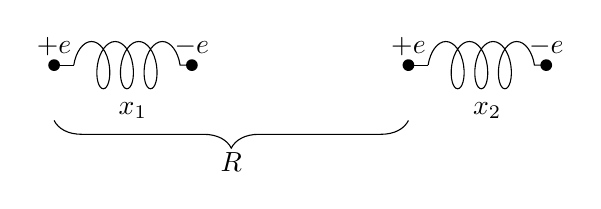
\begin{tikzpicture}
\draw[decoration={aspect=0.5, segment length=3mm, amplitude=3mm,coil},decorate] (0,0) --++ (1.5,0) node[fill=black,inner sep=1.5pt, circle]{} node[above]{$-e$} node[pos=0.5, below,yshift=-1em]{$x_1$};
\draw[] (0,0) --++ (-0.25,0) node[fill=black,inner sep=1.5pt,circle]{} node[above]{$+e$};
\draw[decoration={aspect=0.5, segment length=3mm, amplitude=3mm,coil},decorate] (4.5,0) --++ (1.5,0) node[fill=black,inner sep=1.5pt, circle]{} node[above]{$-e$} node[pos=0.5, below,yshift=-1em]{$x_2$};
\draw[] (4.5,0) --++ (-0.25,0) node[fill=black,inner sep=1.5pt,circle]{} node[above]{$+e$};
\draw[decorate,decoration={brace,amplitude=10pt,mirror},yshift=-20pt] (-0.25,0) -- (4.25,0) node[midway,yshift=-15pt]{$R$};
\end{tikzpicture}
\caption{دو  قابل تقطیب  قریبی جوہر (سوال \حوالہء{6.31})۔}
\label{شکل_غیر_تابع_اضطراب_قابل_تقطیب}
\end{figure}


ان جوہروں کے بیچ کولمب باہم عمل درج ذیل ہوگا 
\begin{align}
H' = \frac{1}{4 \pi \epsilon_0} \big ( \frac{e^2}{R} - \frac{e^2}{R + x_1} - \frac{e^2}{R - x_2} + \frac{e^2}{R + x_1 - x_2} \big )
\end{align}
\begin{enumerate}[a.]
\item
مساوات 6.97 کی تفصیل پیش کریں فاصلہ \عددی{ R} سے \عددی{|x_1|} اور \عددی{|x_2|} کی قیمتوں کو بہت کم تصور کرتے ہوئے درج ذیل دکھائیں 
\begin{align}
H' \cong - \frac{e^2 x_1 x_2}{2 \pi \epsilon_0 R^3}
\end{align}
\item
دکھائیں کے کل ہیملٹنی مساوات 6.96 جمع مساوات 6.98 دو ہارمونی مرتعش ہیملٹن یوں 
\begin{align}
H = \big [ \frac{1}{2m} p_+^2 + \frac{1}{2} \big ( k - \frac{e^2}{4 \pi \epsilon_0 R^3} \big ) x_+^2 \ big ] + \big [ \frac{1}{2m} p_-^2 + \frac{1}{2} \big ( k + \frac{e^2}{4 \pi \epsilon_0 R^3} \big ) x_-^2 \ big ]
\end{align}
میں زیرے تبدیلی متغیرات 
\begin{align} 
X \pm \equiv \frac{1}{\sqrt{2}} (x_1 \pm x_2), \quad \text{\RL{ جس میں}} p \pm =  \frac{1}{\sqrt{2}} (p_1 \pm p_2)
\end{align}
علیحده ہو گا 
\item
اس ہیملٹنی کی زمینی حال توانائی درج ذیل ہوگی 
\begin{align}
E = \frac{1}{2} \hslash (\omega_+ + \omega_- ), \quad \text{RL{ جہاں}} \omega_{\pm} = \sqrt{\frac{k \mp (e^2 / 4 \pi \epsilon_0 R^3)}{m}}
\end{align}
كولمب باہم عمل کے بغیر یہ \عددی{
E_0 = \hslash \omega_0 
} ہوتا جہاں \عددی{
\omega_0 = \sqrt{k /m}
} ہے درج ذیل \عددی{
k \gg (e^2 / 4 \pi \epsilon_0 R^3)
} فرض کرتے ہوئے دکھائیں 
\begin{align}
\Delta V \equiv E - E_0 \cong - \frac{\hslash}{8m^2 \omega_0^3} \big ( \frac{e^2}{4 \pi \epsilon_0} \big )^2 \frac{1}{R^6}
\end{align}
ماخوس: دونوں جوہروں کے بیچ کششی مخفیہ پایا جاتا ہے جو ان کے بیچ فاصلہ کے چھٹی طاقت کے تغیر معکوس ہے یہ دو معدل جوہروں کے بیچ وندر وال باہم عمل ہے 
\item
اسی حساب کو دو رتبی نظریہ اضطراب کی مدد سے دوبارہ کریں اشارہ: غیر مضطرب حالات کی روپ \عددی{
\psi_{n1} (x_1) \psi_{n2} (x_2)
} ہوگی جہاں \عددی{\psi_n(x)} ایک ذرا مرتعش تفاعل موج ہے جہاں \عددی{ m} کمیت اور مقیاس لچک \عددی{k} ہوگا مساوات 6.98 میں دی گئی اضطراب کے لیے زمینی حال توانائی کی دو رتبی تخفیف \عددی{\Delta V} ہوگی دھیان رہے کہ رتبہ اول تخفیف صفر ہے 
\end{enumerate}
\انتہا{سوال}


%what follows is prob 6.32 till the end of the chapter.

سوال6.32:
\\
فرض کریں ایک مخصوص کوانٹم نظام کا  
Hamiltonian 
کسی مقدار معلوم
\(\lambda\)
 کا تفعال ہو .
\(H(\lambda)\)
کے امتیازی اقدار کو اور امتیازی تفعالات
\(E_{n}(\lambda)\)
اور
\(\psi_{n}(\lambda)\)
لیں۔ 
مسلہ Feynman-Hellmann درج ذیل کہتا ہے
\[\frac{\partial E_{n}}{\partial \lambda}=\big\langle{\psi_{n}|\frac{\partial{H}}{\partial{\lambda}}|\psi_{n}}\big\rangle\]
جہاں 
\(E_{n}\)
کو غیر انحطاطی تصور کریں اور اگر انحطاطی ہوں تب تمام 
\(\psi_{n}\)
کو انحطاطی امتیازی تفعالات کے موضوع خطی جوڑ تصور کریں۔\\
(جزو الف):مسلہ Feynman-Hellmann ثابت کریں۔(اشارہ : مسلہ 6.9 استمال کریں ۔ )\\
(جزو ب): درج ذیل یقبودی هارمونی مدار اسکا اطلاق کریں۔\\
ایک)\\
\(\lambda=\omega\)\\
لیں جس سے
V
کی توقعاتی قیمت کا کلیہ اخذ ہوگا ۔\\
دو)\\
\(\lambda=\hslash\)\\
لیں جو
\(\langle T \rangle\)
دے گا اور\\
تین)\\
\(\lambda=m\)\\
جو 
\(\langle T \rangle\)
اور 
\(\langle V \rangle\)
کے درمیان رشتہ دے گا۔اپنے جوابات کا سوال2.12 اور مسلہ virial کی پیشنگویوں  کے ساتھ موعازنا کریں ۔\\
سوال 6.33 : 
\\
مسلہ Feynman-Hellmann استعمال کرتے ہوے ھاٰےڈروجنکے لئے 
\(1/r\)
اور 
\(1/r^{2}\)
کی توقعاتی قیمتیں تین کی جا سکتی ہیں راداسی تفعالات امواج کا موثر 
Hamiltonian 
مساوات 4.53 درج ذیل ہے :
\[H=-\frac{\hslash^{2}}{2m}\frac{d^{2}}{dr^{2}}+\frac{\hslash^{2}}{2m}\frac{l(l+1)}{r^{2}}-\frac{e^{2}}{4\pi\epsilon}\frac{1}{r}\]
اور امتیازی اقدار جنہیں 
L
کی صورت میں لکھا گیا ہے مساوات 4.70 درج ذیل ہونگے 
\[E_n=-\frac{me^{4}}{32\pi^{2}\epsilon^{2}\hslash^{2}(j_{max}+l+1)^{2}}\]
(جزو الف):\\
 مسلہ Feynman-Hellmann میں 
\(\lambda=e\)
استعمال کرتے ہوے
\(\langle1/r\rangle\)
تلاش کریں۔ اپنے نتیجے کی تصدیق مساوات 6.55 کے ساتھ کریں۔\\
(جزو ب) :\\
\(\lambda=l\)
کو استعمال کرتے ہوے
\(\langle1/r^{2}\rangle\)
تلاش کریں۔ اپنے نتیجے کی تصدیق مساوات 6.56 کے ساتھ کریں۔\\
سوال 6.34 :\\
 رشتہ Kramers' 
\[\frac{s+1}{n^{2}}\langle r^{s}\rangle -(2s+1)a\langle r^{s-1}\rangle n+\frac{s}{4}[(2l+1)^{2}-s^{2}]a^{2}\langle r^{s-2}\rangle =0\]
صابط کریں جو ھاٰےڈروجنکےحال 
\(\psi_{nlm}\)
میں الیکٹران کے لئے R کی توقعاتی قیمتوں کی تین مختلف طاقتوں
\((s,s-1,\)
اور
\(s-2)\)
کا۔ تعلق پیش کرتا ہے۔ اشارہ : راداسی مساوات 4.53 کو درج ذیل روپ میں لکھ کر
\[u''=\big[\frac{l(l+1)}{r^{2}}-\frac{2}{ar}+\frac{1}{n^{2}a^{2}}\big]u.\]
۔
\(\int(ur^{s}u'')dr\)	 
کو 
\(\langle r^{s}\rangle\)
،
\(\langle r^{s-1}\rangle\)
،
\(\langle r^{s-2}\rangle \)
کی  صورت میں لکھیں اسکے بعد تکامل
bilhisis
کے ذریےدوہرا تفروق کو بیٹھایں۔ دیکھایں کے\\
\[\int(ur^{s}u')=-(s/2)<r^{s-1}>\]
اور
\[\int(u'r^{s}u')dr=-[2/(s+1)]\int(u''r^{s+1}u')dr\]
ہوگا اسی کو لے کر آگے چلیں)\\
سول 6.35\\ 
(جزو الف ):\\
 رشتہ Kramers' مساوات 6.104 میں
\(s=0,s=1,s=2\)
اور 
\(s=3\)
ڈال کے 
\(\langle r^{-1}\rangle,\langle r\rangle,\langle r^{2}\rangle\)
اور 
\(\langle r^{3}\rangle\)
کے قلیات حاصل کریں۔ آپ دیکھ سکتے ہیں کے آپ اس طرح چلتے ہے کسی بھی مثبت طاقت کے لئے قلیہ دریافت کر سکتے ہیں ۔\\
(جزو ب):\\ 
دوسرے رخ آپکو مثلا درپیش  ہوگا آپ 
\(s=-1\)
پر کرکے دیکھیں کے آپکو صرف 
\(\langle r^{-2}\rangle\)
اور 
\(\langle r^{-3}\rangle\)
کے بیچ رشتہ حاصل ہوگا ۔\\
جزو ج:\\
 اگر آپ کسی طریقہ سے
\(\langle r^{-2}\rangle\)
دریافت کر پایں تب آپ رشتہ Kramers' استعمال کرکے باکی تمام منفی قوعتوں کے لئے قلیات دریافت کر سکتے ہیں ۔\\
مساوات 6.56 : جسے سوال 6.33 میں اخذ کیا گیا ہے اسے استعمال کرتے ہوے 
\(\langle r^{-3}\rangle\)
تعین کریں اور اپنے نتیجہ کی تصدیق مساوات 6.64 کے ساتھ کریں۔\\
سوال 6.36: \\
ایک جوہر کو يقسا بیرونی برقی میدان
\(E_{ext}\)
میں رکھنے سے توانائی کی سطحیں بٹتی ہیں جسے سٹارک اثر کہا جاتا ہے اور جو zemann اثر کا برقی مماسل ہے اس سوال میں ہم ھاٰےڈروجن کے 
\(n=1\)
اور 
\(n=2\)
حالات کے لئے سٹارک اثر کا تجزیہ کرتے ہیں۔ فرض کریں میدان
Z
رخ ہے لہٰذا الیکٹران کی مخفی توانائی درج ذیل ہوگی: 
\[H'_{S}=eE_{ext}z=eE_{ext}r\cos{\theta}\]
اسکو bohr hamiltonian  مساوات 6.42 میں اضطراب تصور کریں اس مسلہ میں چکر کا کوئی کردار نہیں ہے لہذا اسے نظر انداز کرتے ہوے عمدہ ساخت کو رعد کریں۔\\
(جزو الف ) :\\
 اول رتبہ میں زمینی حال توانائی اس اضطراب سے اثر انداذ نہیں ہوتی ۔\\
(جزو ب) :\\  
پہلا هیجان حال
4
پرتہ
\(\psi_{200},\psi_{211},\psi_{210},\psi_{21-1},\)
انحطاطی نظریہ اضطراب استعمال کرتے ہوے، توانائی کی رتبہِ اول کا سہی تعین کریں ۔توانائی 
\(E_{2}\)
کتنے سطحوں میں بٹے گا؟\\
(جزو ج) :\\
 درج بالہ جزو ب میں موضوع تفعالات موج کیا ہونگے ؟ ان میں سے ہر ایک موضوع حالات میں برقی جوعف قطب میعارِاثر
\((p_{e}=-er)\)
کی توقعاتی قیمت معلوم کریں ۔ آپ دیکھیں گے کہ نتائج  لاگو میدان کے تعابع نہیں ہونگے اس طرح ظاہر ہے کے پہلی هیجان حال میں ھاٰےڈروجن برقی جوعفت قطب میعارِاثر کا حامل ہوگا۔اشارہ:اس سوال میں بہت سارے تاكملات پاے جاتے ہیں تاہم تقریبن تمام کی قیمت سِفر ہے لہذا حساب سے قبل غور کریں اگر 
\(\phi\)
تكمل سفر ہو تب 
\(r\)
اور 
\(\theta\)
تکملات حل کرنے  کی ضرورت نہیں ہوگی جزوی جواب
\[W_{13}=W_{31}=-3eaE_{ext};\]
باقی تمام ارکان سفر ہیں۔ )\\
سوال 6.37:
 ھاٰےڈروجن کی 
\(n=3\)
حالات کے لئے سٹارک  اثر سوال 6.36 پر غور کریں ابتدائ طور پر چکر کو نظر انداز کرتے ہوے اب انحطاطی حالات 
\(\psi_{3lm}\)
ہونگے اور اب ہم 
\(z\)
رخ برقی میدان چالو کرتے ہیں ۔\\
(جزو الف) :\\ 
اضطرابی hamiltonian کو ظاہر کرنے والا 
\(9\times9\)
کا کالم  تیار کریں\\
 جزوی جواب 
\[\langle 300|z|310\rangle =-3\sqrt{6}a,\langle 310|z|320\rangle =-3\sqrt{3}a,\langle 31\pm1|z|32\pm1\rangle=-(9/2)a.\]\\
(جزو ب) :\\ 
امتیازی اقتدار اور انکی انحطاط دریافت کریں .\\
سوال 6.38 :
  ڈوٹرئم
کی زمینی حال میں نہایت موحین منتقلی کے دوران خارج کردہ پھوٹان کا طولِ موج
میں تلاش کریں ۔ ڈوٹرئم درحقیقت بھاری ھاٰےڈروجن ہے جسکے مرکز میں ایک اضافی نوٹران پایا جاتا ہے پروٹان اور نوٹران ساتھ جڑ کر  ڈوٹرئم بناتے ہیں جسکا چکر ایک مقناطیسی دارِاثر
\[\mu_{d}=\frac{g_{d}e}{2m_{d}}S_{d};\]
اور ڈوٹرئم کا 
g-
جزو 1.71 ہے ۔\\
سوال 6.39 :\\
 ایک کالم میں قریبی باردارا کا بجلی میدان جوہر کی توانائی کی سطحوں کو مضطرب کرتا ہے۔ ایک تازہ نمونہ کے طور پر   (شکل \حوالہ{شکل_غیر_تابع_اضطراب_قلمی_جال})   فرض کریں  ہائیڈروجن  جوہر کی پڑوس میں نقطہ باروں کی تین جوڑیاں پای جاتی ہیں ۔(چونکے اس۔ سوال کے ساتھ چکر کا کوئی۔ واستہ نہیں ہے لہٰذا اسے نظرانداز کریں )
 
 \begin{figure}
\centering
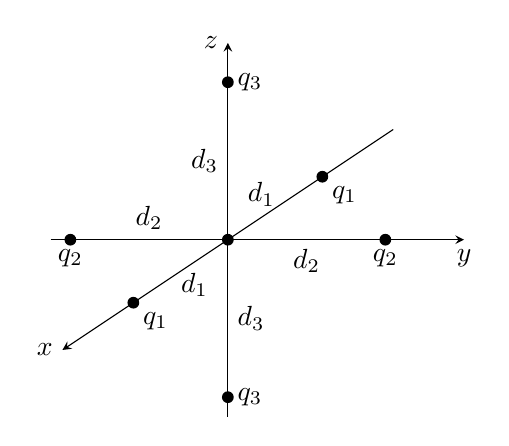
\begin{tikzpicture}[x={(-0.6cm,-0.4cm)},y={(1cm,0cm)},z={(0cm,1cm)}]
\draw[-stealth](0,-2.25,0) -- (0,3,0) node[below]{$y$};
\draw[-stealth](-3.5,0,0) -- (3.5,0,0) node[left]{$x$};
\draw[-stealth](0,0,-2.25) -- (0,0,2.5) node[left]{$z$};
\draw[](-2,0,0) node[fill=black,inner sep=1.5pt,circle]{} node[below right]{$q_1$};
\draw[](2,0,0) node[fill=black,inner sep=1.5pt,circle]{} node[below right]{$q_1$};
\draw[](0,-2,0) node[fill=black,inner sep=1.5pt,circle]{} node[below]{$q_2$};
\draw[](0,2,0) node[fill=black,inner sep=1.5pt,circle]{} node[below]{$q_2$};
\draw[](0,0,-2) node[fill=black,inner sep=1.5pt,circle]{} node[right]{$q_3$};
\draw[](0,0,2) node[fill=black,inner sep=1.5pt,circle]{} node[right]{$q_3$};
\draw[] (-1,0,0) node[shift={(-5pt,5pt)}]{$d_1$};
\draw[] (1,0,0) node[shift={(5pt,-5pt)}]{$d_1$};
\draw[] (0,-1,0) node[above]{$d_2$};
\draw[] (0,1,0) node[below]{$d_2$};
\draw[] (0,0,-1) node[right]{$d_3$};
\draw[] (0,0,1) node[left]{$d_3$};
\draw(0,0,0) node[circle,fill=black,inner sep=1.5pt]{};
\end{tikzpicture}
\caption{ہائیڈروجن جوہر کے گرد   چھ نقطی بار (قلمی جال کا ایک سادہ نمونہ)؛ سوال \حوالہء{6.39}}
\label{شکل_غیر_تابع_اضطراب_قلمی_جال}
\end{figure}

(جزو الف ):\\
 درج ذیل 
\[r<<d_{1},r<<d_{2},andr<<d_{3},\]
کی صورت میں دیکھاے
\[H'=V_{o}+3(\beta_{1}x^{2}+\beta_{2}y^{2}+\beta_{3}z^{2})-(\beta_{1}+\beta_{2}+\beta_{3})r^{2},\]
جہاں  درج ذیل ہیں
\[\beta_{i}\equiv-\frac{e}{4\pi\epsilon}\frac{\eta_{i}}{d_{i}^{3}},\quad\quad\]
اور 
\[V_{o}=2(\beta_{1}d_{1}^{2}+\beta_{2}d_{2}^{2}+\beta_{3}d_{3}^{2}).\]\\
(جزو ب) : \\زمینی حال توانائی کی رتبا اول کی تخفیف تلاش کریں ۔\\
(جزو ج) :\\ پہلی۔ هیجان حالات 
\((n=2)\)
کی توانائی کے لئے رتبااول کی تخفیف تلاش کریں ۔ درجذیل صورتوں میں یہ چار پڑتہ انحطاطی نظام کتنی سطحوں میں بٹے گا ۔\\
ایک ) کابی تشاقلی
\[\beta_{1}=\beta_{2}=\beta_{3},\]
کی۔ صورت میں ۔\\
دو ) چوں زاویہ تشاقلی
\[\beta_{1}=\beta_{2}\neq\beta_{3}:\]
کی صورت میں۔\\
تین ) آرتھو ھامبک تشاقل کی صورت میں تینوں مختلف ہونگیں ۔\\
سوال 6.40 : \\بازاوقات 
\(\psi_{n}^{1}\)
کو غیر مضطرب طفعالات امواج میں پهلاۓ  مساوات 6.11 بغیر مساوات 6.10 کو بلہ واستہ حال کرنا ممکن ہوتا ہے اسکی دو بلخصوص خوبصورت مثالین درج ذیل ہیں۔\\
(الف )\\
ایک) ھاٰےڈروجن کی زمینی حال میں سٹارک اثر ایک یکساں بیرونی برقی میدان 
\(E_{ext}\)
کی۔ موجودگی میں ھاٰےڈروجن  کی زمینی حال کا رتبہ اول تخفیف تلاش کریں ( سوال 6.36 stark اثر دیکھیں ۔) ۔اشارہ : حل کی درج ذیل روپ :\\
\[(A+Br+Cr^{2})e^{-r/n}cos\theta;\]
استعمال کرکے دیکھیں اپ نے مستقلات 
\(A,B,\)
اور 
\(C\)
کی ایسی قیمتیں تلاش کرنی ہیں جو مساوات 6.10 کو مطمئن کرتے ہوں ۔\\
دو ) زمینی حال توانائی کی رتبہ دوم تخفیف مساوات 6.14 کی مدد سے  تعین کریں جیسا اپنے سوال 6.36 (الف ) میں دیکھا رتبہ اول تخفیف سفر ہوگی ۔جواب :\\
\[-m(3a^{2}eE_{ext}/2\hslash)^{2}.\]\\
(جزو ب)\\ اگر پروٹان کا برقی جست قطب میعارِاثر 
\(p\)
ہوتا تب  ھاٰےڈروجن کے  الیکٹرانکی مخفی توانائی درجذیل مقدار سے مضطرب ہوتی۔
\[H'=\frac{epcos\theta}{4\pi\epsilon r^{2}}\]
ایک ) زمینی حال طفعال موج کی رتبی اول تخفیف کو مساوات 6.10 حل کرکے تلاش کریں ۔\\
دو ) دیکھایں کہ رتبہ تک جوہر کا قل برقی جوعفت قطب میعارِاثر حیرت کی۔ بات ہے سفر ہوگا۔ \\
تین ) زمینی حال توانائی کی۔ رتبہ دوم تخفیف مساوات 6.14 سے تعین کریں رتبہ اول تخفیف کیا ہوگا ؟\\
\\

